
% Template for Elsevier CRC journal article
% version 1.1 dated 16 March 2010

% This file (c) 2009-10 Elsevier Ltd.  Modifications may be freely made,
% provided the edited file is saved under a different name

% This file contains modifications for Nuclear Physics B Proceedings Supplement

% Changes since version 1.0
% - elsarticle class option changed from 1p to 3p (to better reflect CRC layout)
%

%-----------------------------------------------------------------------------------

%% This template uses the elsarticle.cls document class and the extension package ecrc.sty
%% For full documentation on usage of elsarticle.cls, consult the documentation "elsdoc.pdf"
%% Further resources available at http://www.elsevier.com/latex

%-----------------------------------------------------------------------------------

%%%%%%%%%%%%%%%%%%%%%%%%%%%%%%%%%%%%%%%%%%%%%%
%%%%%%%%%%%%%%%%%%%%%%%%%%%%%%%%%%%%%%%%%%%%%%
%%                                          %%
%% Important note on usage                  %%
%% -----------------------                  %%
%% This file must be compiled with PDFLaTeX %%
%% Using standard LaTeX will not work!      %%
%%                                          %%
%%%%%%%%%%%%%%%%%%%%%%%%%%%%%%%%%%%%%%%%%%%%%%
%%%%%%%%%%%%%%%%%%%%%%%%%%%%%%%%%%%%%%%%%%%%%%

%% The '3p' and 'times' class options of elsarticle are used for Elsevier CRC
\documentclass[3p,times,twocolumn]{elsarticle}

%% The `ecrc' package must be called to make the CRC functionality available
\usepackage{ecrc}

%% The ecrc package defines commands needed for running heads and logos.
%% For running heads, you can set the journal name, the volume, the starting page and the authors

%% set the volume if you know. Otherwise `00'
\volume{00}

%% set the starting page if not 1
\firstpage{1}

%% Give the name of the journal
\journalname{Nuclear Physics B Proceedings Supplement}

%% Give the author list to appear in the running head
%% Example \runauth{C.V. Radhakrishnan et al.}
\runauth{}

%% The choice of journal logo is determined by the \jid and \jnltitlelogo commands.
%% A user-supplied logo with the name <\jid>logo.pdf will be inserted if present.
%% e.g. if \jid{yspmi} the system will look for a file yspmilogo.pdf
%% Otherwise the content of \jnltitlelogo will be set between horizontal lines as a default logo

%% Give the abbreviation of the Journal.
\jid{nuphbp}

%% Give a short journal name for the dummy logo (if needed)
\jnltitlelogo{Nuclear Physics B Proceedings Supplement}

%% Hereafter the template follows `elsarticle'.
%% For more details see the existing template files elsarticle-template-harv.tex and elsarticle-template-num.tex.

%% Elsevier CRC generally uses a numbered reference style
%% For this, the conventions of elsarticle-template-num.tex should be followed (included below)
%% If using BibTeX, use the style file elsarticle-num.bst

%% End of ecrc-specific commands
%%%%%%%%%%%%%%%%%%%%%%%%%%%%%%%%%%%%%%%%%%%%%%%%%%%%%%%%%%%%%%%%%%%%%%%%%%

%% The amssymb package provides various useful mathematical symbols
\usepackage{amssymb}
%% The amsthm package provides extended theorem environments
%% \usepackage{amsthm}

%% The lineno packages adds line numbers. Start line numbering with
%% \begin{linenumbers}, end it with \end{linenumbers}. Or switch it on
%% for the whole article with \linenumbers after \end{frontmatter}.
%% \usepackage{lineno}

%% natbib.sty is loaded by default. However, natbib options can be
%% provided with \biboptions{...} command. Following options are
%% valid:

%%   round  -  round parentheses are used (default)
%%   square -  square brackets are used   [option]
%%   curly  -  curly braces are used      {option}
%%   angle  -  angle brackets are used    <option>
%%   semicolon  -  multiple citations separated by semi-colon
%%   colon  - same as semicolon, an earlier confusion
%%   comma  -  separated by comma
%%   numbers-  selects numerical citations
%%   super  -  numerical citations as superscripts
%%   sort   -  sorts multiple citations according to order in ref. list
%%   sort&compress   -  like sort, but also compresses numerical citations
%%   compress - compresses without sorting
%%
%% \biboptions{comma,round}

% \biboptions{}

% if you have landscape tables
\usepackage[figuresright]{rotating}

% put your own definitions here:
% particles
\newcommand{\PH}{\ensuremath{\mathrm{H}}}
\newcommand{\V}{\ensuremath{\mathrm{V}}}
\newcommand{\PZ}{\ensuremath{\mathrm{Z}}}
\newcommand{\PW}{\ensuremath{\mathrm{W}}}
\newcommand{\PWm}{\ensuremath{\mathrm{W^-}}}
\newcommand{\PWp}{\ensuremath{\mathrm{W^+}}}
\newcommand{\Pgg}{\ensuremath{\gamma}}
\newcommand{\Pgs}{\ensuremath{\gamma^*}}
\newcommand{\Pg}{\ensuremath{\mathrm{g}}} % generic gluon
\newcommand{\Pe}{\ensuremath{\mathrm{\mathrm{e}}}}
\newcommand{\Pep}{\ensuremath{\mathrm{\mathrm{e}}^{+}}}
\newcommand{\Pem}{\ensuremath{\mathrm{\mathrm{e}}^{-}}}
\newcommand{\Pepm}{\ensuremath{\mathrm{\mathrm{e}}^{\pm}}}
\newcommand{\Pemp}{\ensuremath{\mathrm{\mathrm{e}}^{\mp}}}
\newcommand{\Pm}{\ensuremath{\mu}}
\newcommand{\Pmp}{\ensuremath{\mu^{+}}}
\newcommand{\Pmm}{\ensuremath{\mu^{-}}}
\newcommand{\Pmpm}{\ensuremath{\mu^{\pm}}}
\newcommand{\Pmmp}{\ensuremath{\mu^{\mp}}}
\newcommand{\Pq}{\ensuremath{\mathrm{q}}}
\newcommand{\Paq}{\ensuremath{\mathrm{\overline{q}}}}

\newcommand{\X}{\ensuremath{\mathrm{X}}}

% channels
\newcommand{\chanHZZ}{\ensuremath{\PH\to\PZ\PZ\to4\ell}}
\newcommand{\chanHWW}{\ensuremath{\PH\to\PW\PW\to\ell\nu\ell\nu}}
\newcommand{\chanHgg}{\ensuremath{\PH\to\Pgg\Pgg}}
\newcommand{\qqbar}{\ensuremath{\mathrm{\Pq\Paq}} }
\newcommand{\wgamma}{\ensuremath{\PW\Pgg}}
\newcommand{\wjets}{\ensuremath{W+}jets} 
\newcommand{\tw}{\ensuremath{\mathrm{t}\PW}} 
\newcommand{\ttbar}{\ensuremath{\mathrm{t}\overline{\mathrm{t}}}} % t-tbar

% units
%\newcommand{\fbinv}{\ensuremath{fb^{-1}}}
\newcommand{\fbinv}{\ensuremath{\,\mathrm{fb}^\mathrm{-1}}}
\newcommand{\GeV}{\ensuremath{\,\mathrm{Ge\hspace{-.08em}V}}}
\newcommand{\TeV}{\ensuremath{\,\mathrm{Te\hspace{-.08em}V}}}

% kinematics
\newcommand{\PT}{\ensuremath{p_{\mathrm{T}}}}
\newcommand{\pt}{\ensuremath{p_{\mathrm{T}}}}
\newcommand{\ET}{\ensuremath{E_{\mathrm{T}}}}
\newcommand{\HT}{\ensuremath{H_{\mathrm{T}}}}
\newcommand{\et}{\ensuremath{E_{\mathrm{T}}}}
\newcommand{\PTm}{\ensuremath{{p}_\mathrm{T}\hspace{-1.02em}/\kern 0.5em}}
\newcommand{\PTslash}{\PTm}
\newcommand{\ETm}{\ensuremath{E_{\mathrm{T}}^{\mathrm{miss}}}}
\newcommand{\MET}{\ETm}
\newcommand{\ETmiss}{\ETm}
\newcommand{\ETslash}{\ensuremath{E_{\mathrm{T}}\hspace{-1.1em}/\kern0.45em}}
\newcommand{\VEtmiss}{\ensuremath{{\vec E}_{\mathrm{T}}^{\mathrm{miss}}}}
\newcommand{\ptvec}{\ensuremath{{\vec p}_{\mathrm{T}}}}
\newcommand{\met}{\ETm}
\newcommand{\vmet}{\ensuremath{\vec{E}_\mathrm{T}}^{\mathrm{miss}}}
\newcommand{\mth}{\ensuremath{m_{\mathrm{T}}}}
\newcommand{\mll}{\ensuremath{m_{\ell\ell}}}
\newcommand{\delphillmet}{\ensuremath{\Delta\phi(\ell\ell,\vec{E}_\mathrm{T}^{\mathrm{miss}})}}
\newcommand{\ptll}{\ensuremath{\pt^{\ell\ell}}}
\newcommand{\mgg}{\ensuremath{m_{\gamma\gamma}}}
\newcommand{\ptgg}{\ensuremath{p_{\mathrm{T}}^{\gamma\gamma}}}


% softwares and MC
\newcommand{\MCFM} {\textsc{mcfm}}
\newcommand{\JHUGEN} {\textsc{JHUGen}}

% kinematic discriminants
\newcommand{\KD}{\ensuremath{{\cal D}^{\rm kin}_{\rm bkg}} }
\newcommand{\superKD}{\ensuremath{{\cal D}_{\rm bkg}} }
\newcommand{\spinKD}{\ensuremath{{\cal D}_{J^P}} }
\newcommand{\psvectorKD}{\ensuremath{{\cal D}_{1^-}} }
\newcommand{\vectorKD}{\ensuremath{{\cal D}_{1^+}} }
\newcommand{\zerominusKD}{\ensuremath{{\cal D}_{\rm 0^-}} }
\newcommand{\zerohplusKD}{\ensuremath{{\cal D}_{\rm 0_h^+}} }
\newcommand{\lambdaKD}{\ensuremath{{\cal D}_{\Lambda_{1}}} }
\newcommand{\interfzerominusKD}{\ensuremath{{\cal D}_{\rm bkg}^{SM,{0^-}}} }
\newcommand{\interfzerohplusKD}{\ensuremath{{\cal D}_{\rm bkg}^{SM,{0_h^+}}} }
\newcommand{\VDj}{\mathrm{{\cal D}_{\rm jet}} }
\newcommand{\VDu}{\mathrm{{\cal D}_{\PT}} }
\newcommand{\MassD}{\mathrm{{\cal D}_{\rm mass}} }
\newcommand{\costhetastar}{\ensuremath{\cos\theta^{\ast}_{\mbox{\tiny{CS}}}}}
\newcommand{\abscostheta}{\ensuremath{|{\cos\theta^{\ast}_{\mbox{\tiny{CS}}}}|}}
% fonts
\def\sss{\scriptscriptstyle}


% add words to TeX's hyphenation exception list
%\hyphenation{author another created financial paper re-commend-ed Post-Script}

% declarations for front matter

\begin{document}

\begin{frontmatter}

%% Title, authors and addresses

%% use the tnoteref command within \title for footnotes;
%% use the tnotetext command for the associated footnote;
%% use the fnref command within \author or \address for footnotes;
%% use the fntext command for the associated footnote;
%% use the corref command within \author for corresponding author footnotes;
%% use the cortext command for the associated footnote;
%% use the ead command for the email address,
%% and the form \ead[url] for the home page:
%%
%% \title{Title\tnoteref{label1}}
%% \tnotetext[label1]{}
%% \author{Name\corref{cor1}\fnref{label2}}
%% \ead{email address}
%% \ead[url]{home page}
%% \fntext[label2]{}
%% \cortext[cor1]{}
%% \address{Address\fnref{label3}}
%% \fntext[label3]{}

\dochead{}
%% Use \dochead if there is an article header, e.g. \dochead{Short communication}

\title{Studies of the Higgs boson spin and parity using the $\gamma\gamma$, ZZ, and WW decay channels with the CMS detector}

%% use optional labels to link authors explicitly to addresses:
%% \author[label1,label2]{<author name>}
%% \address[label1]{<address>}
%% \address[label2]{<address>}

\author{Emanuele Di Marco}

\address{CERN, CH-1211 Geneva 23, Switzerland}

\begin{abstract}
Studies of the Higgs boson spin and parity are presented using data
samples corresponding to the $\gamma\gamma$, ZZ, and WW decay
channels. The analyses are based on pp collision data collected at
centre-of-mass energies of 7 and 8 TeV, corresponding to integrated
luminosities of approximately 5$\fbinv$ and 20$\fbinv$, respectively. The data
are compared to the expectations for a Standard Model Higgs boson, and
for several alternative models.
\end{abstract}

\begin{keyword}
%% keywords here, in the form: keyword \sep keyword
  
%% MSC codes here, in the form: \MSC code \sep code
%% or \MSC[2008] code \sep code (2000 is the default)

\end{keyword}

\end{frontmatter}

%%
%% Start line numbering here if you want
%%
% \linenumbers

%% main text
\section{Introduction}
\label{sec:introduction}
The observation of a new boson~\cite{Aad:2012tfa,Chatrchyan:2012ufa}
with a mass around $125\GeV$ and properties consistent with the
standard model (SM) Higgs boson was reported by the ATLAS and CMS
Collaborations in 2012. The discovery was followed by an extensive set
of measurements of its properties to determine if they follow the SM
predictions or if there are indications for physics beyond the SM
(BSM). The decays of this boson into two electroweak (EW) gauge
bosons, $\chanHZZ$, $\chanHWW$, $\chanHgg$, can provide information on
the consiustency of its spin-parity with the hypothesis of a spin-zero
scalar SM Higgs boson.

In this conference I reported the results on the Higgs boson
spin-parity properties and tensor structure interactions with EW gauge
bosons using the $\PH\to\PZ\PZ$, $\PZ\Pgs$, $\Pgs\Pgs\to4\ell$,
$\chanHWW$ decay modes, with $\ell=\Pepm,\Pmpm$. The results are
presented in terms of constraints on the anomalous coupling
contributions to the $\PH$VV interactions for the spin-zero
assumption, and exclusion of exotic spin-one and spin-two states.  By
using the $\PH\to\Pg\Pg$ decay channel, the exotic spin-two scenario
can be further constrained.  For the studies presented, the full Run1
LHC data sample collected by CMS experiment at 7 and 8 $\TeV$ is used.




\section{Phenomenology of anomalous HVV interactions}
\label{sec:phenomenology}
For the studies presented, the formalism of the scattering amplitude is used
to describe the interactions of a boson $\PH$ with a pair of vector bosons $\V_1$ and $\V_2$.

\subsection{Spin-zero resonance}
For a spin-zero boson $\PH$ and two spin-one gauge bosons $\V\V$, such
as $\PZ\PZ, \PZ \Pgg, \Pgg\Pgg, \PW\PW$, or $\Pg\Pg$, the scattering amplitude
presents three invariant tensor terms with coupling complex constants $a_{i}^{\V\V}$
which in general can depend on the Lorentz invariant four-momenta
of $\V_1$ and $\V_2$ squared, $q_{\sss\V1}^2$ and $q_{\sss\V2}^2$. 
In the following, the terms up to $q_{\sss\V}^2$  are kept in the expansion under the assumption 
of small contributions from anomalous couplings
%
\begin{eqnarray}
A(\PH\V\V) \sim 
\left[ a_{1}^{\V\V} 
+ \frac{\kappa_1^{\V\V}q_{\sss\V1}^2 + \kappa_2^{\V\V} q_{\sss\V2}^{2}}{\left(\Lambda_{1}^{\V\V} \right)^{2}} \right] 
m_{\sss\V1}^2 \epsilon_{\sss\V1}^* \epsilon_{\sss\V2}^* \\ \nonumber
+ a_{2}^{\V\V}  f_{\mu \nu}^{*(1)}f^{*(2),\mu\nu} 
+ a_{3}^{\V\V}   f^{*(1)}_{\mu \nu} {\tilde f}^{*(2),\mu\nu}\,,
\label{eq:formfact-fullampl-spin0} 
\end{eqnarray}
%
where $f^{(i){\mu \nu}} =
\epsilon_{{\sss\V}i}^{\mu}q_{{\sss\V}i}^{\nu} -
\epsilon_{{\sss\V}i}^\nu q_{{\sss\V}i}^{\mu} $ is the field strength
tensor of a gauge boson with momentum $q_{{\sss\V}i}$ and polarization
vector $\epsilon_{{\sss\V}i}$, ${\tilde f}^{(i)}_{\mu \nu} =
\frac{1}{2} \epsilon_{\mu\nu\rho\sigma} f^{(i),\rho\sigma}$ is the
dual field strength tensor, the superscript~$^*$ designates a complex
conjugate, $m_{\sss\V1}$ is the pole mass of the vector boson $\PZ$ or
$\PW$, and $\Lambda_{1}$ is the scale of BSM physics and is a free
parameter of the model~\cite{Anderson:2013afp}. The tree-level SM-like
contribution corresponds to $a_{1}^{\PZ\PZ}\ne 0$ and $a_{1}^{\PW\PW}
\ne 0$, while there is no tree-level coupling to massless gauge
bosons, that is $a_{1}^{\V\V}= 0$ for $\PZ \gamma, \gamma\gamma$, and
$\Pg\Pg$. The other terms in the SM can be generated through loop
effects, and are expected to be small enough to be observed with the
current LHC dataset, thus they are considered as anomalous couplings.

The parity-conserving interaction of a pseudoscalar ($CP$-odd state)
corresponds to the $a_{3}^{\V\V}$ terms, while the other terms
describe the parity-conserving interaction of a scalar ($CP$-even
state).  The $a_{3}^{\V\V}$ terms appear in the SM only at a
three-loop level and receive a small contribution.  The $a_{2}^{\V\V}$
and $\Lambda_{1}^{\V\V}$ terms appear in loop-induced processes and
also give small contributions $O(10^{-3} - 10^{-2})$.

Contributions from BSM particles can change both the magnitude and the
phases of these couplings, given their non-trivial dependence on the
Lorentz invariant quantities. When the particles in the loops
responsible for these couplings are heavy in comparison to the Higgs
boson mass, the couplings are real.  The scenarios are parameterized
in terms of the effective fractional cross sections and their phases
with respect to the two dominant tree-level couplings $a_1$ and
$a_1^{\PW\PW}$ in the $\PH\to \V\V\to 4\ell$ and $\PH\to \PW\PW\to
\ell\nu\ell\nu$ processes, respectively:
$(f_{\Lambda1},\phi_{\Lambda1})$, $(f_{a2}, \phi_{a2} =
\mathrm{arg}\left(\frac{a_{2}}{a_{1}}\right))$, $(f_{a3},\phi_{a3} =
\mathrm{arg}\left(\frac{a_{3}}{a_{1}}\right))$.  The couplings of the
Higgs boson to $\PZ\Pgg$ and $\Pgg\Pgg$ are also accessible in these
decays and can be measured with the same techniques in the
$\PH\to4\ell$ decays, but with the current LHC dataset they are much
better constrained via the decays on the on-shell gauge bosons.

The couplings in the $\chanHZZ$ and $\chanHWW$ decay channels can be
related with functions of two free parameters. If $f_{ai}$ is the
fraction in the $\PH\PZ\PZ$ coupling, then the other parameter can be
expressed in terms of the ratio of the anomalous couplings of the two
channels:
%
\begin{eqnarray}
r_{ai} = \frac{a_i^{\PW\PW} / a_1^{\PW\PW}  }{  a_i / a_1}\,, ~~{\rm or}~~~ R_{ai} = \frac{ r_{ai} |r_{ai}| }{  1 + r_{ai}^2 }  \, .
\label{eq:ratio_ww_zz}
\end{eqnarray} 
%
%% and the combination of $f_{ai}$ in the two channels is viable through the relationship:
%% %
%% \begin{eqnarray}
%% f_{ai} = \left[ 1+r_{ai}^2(1/f_{ai}^{\PW\PW}-1)\sigma_{i}^{\PW\PW}\sigma_{1}/(\sigma_{1}^{\PW\PW}\sigma_{i}) \right]^{-1}
%% \,.
%% \label{eq:a2_conversion}
%% \end{eqnarray}
%% %
%
A more complete description of the phenomenology of $\PH\V\V$
anomalous interactions can be found in Ref.\cite{CMS:2014gga}.


\subsection{Exotic spin-one and spin-two resonance}
A spin-one resonance cannot decay into $\Pgg\Pgg$ final state because
of the Landau-Yang theorem. We anyway tested this hypothesis for the
$\PZ\PZ$ and $\PW\PW$ channels, assuming the existence of two states
that decay in different channels. We test the spin-two hypothesis for
all the three channels.  The scattering amplitude of the exotic boson
with spin one ($X_{J=1}$) consists of two independent terms, which can
be written as
%
\begin{eqnarray}
A(\X_{J=1} \V\V) \sim b_{1}^{\V\V}  \left[ \left(\epsilon_{\sss\V1}^{*}q\right)\left(\epsilon_{\sss\V2}^{*}\epsilon_{\sss\X}\right) +
\left(\epsilon_{\sss\V2}^{*}q\right)\left(\epsilon_{\sss\V1}^{*}\epsilon_{\sss\X}\right) \right] + \\ \nonumber 
b_{2}^{\V\V}  \epsilon_{\alpha\mu\nu\beta}\epsilon_{\sss\X}^{\alpha}\epsilon_{\sss\V1}^{*\mu}\epsilon_{\sss\V2}^{*\nu}{\tilde q}^{\beta} \,,
\label{eq:ampl-spin1} 
\end{eqnarray}
%
where $\epsilon_{\sss\X}$ is the polarization vector of the boson $\X$
with spin one, ${q}=q_{\sss\V1}+q_{\sss\V2}$ and ${\tilde
  q}=q_{\sss\V1}-q_{\sss\V2}$~\cite{Gao:2010qx, Bolognesi:2012mm}.
Here the $b_{1}^{\V\V} \neq 0$ coupling corresponds to a vector
particle, while the $b_{2}^{\V\V}\neq 0$ coupling corresponds to a
pseudovector particle.  As in the case of spin-zero resonance, we
define a continuous parameter that describes the presence of the
corresponding terms $b_{1}^{\V\V} $ and $b_{2}^{\V\V}$ as an effective
fractional cross section $f_{b2}^{\V\V}$.  The $f_{b2}^{\V\V}$
parameter is used to test if the data favors the SM Higgs boson scalar
hypothesis or some particular mixture of the vector and pseudovector
states.

The scattering amplitude for a spin-two boson is more complex and its
expression can be found in \cite{CMS:2014gga}.  It contains ten
complex terms, and they are fully tested in this study.  In this case
we consider both the decays into massive gauge bosons, $\PZ\PZ$ or
$\PW\PW$, and to two on-shell photons, $\X\to\Pgg\Pgg$. Both $\qqbar$
production and gluon fusion, spin-two state are considered for the
$\PH\to4\ell$ final states. The set of models considered are: $2_m^+$,
$2_{h2}^+$, $2_{h3}^+$, $2_h^+$, $2_b^+$, $2_{h6}^+$, $2_{h7}^+$,
$2_h^-$, $2_{h9}^-$, $2_{h10}^-$.  The subscripts $m$ (minimal
couplings), $h$ (couplings with higher-dimension operators), and $b$
(bulk) distinguish different scenarios.  In the case of the $\Pgg\Pgg$
decay only the results for a massive graviton-like boson, $2_m^+$ are
considered.


\section{Kinematic observables}
\label{sec:observables}
The measurements of the spin-parity properties of the Higgs boson make
use of the kinematics of the four leptons in the event, for the
$\PH\to\V\V$ channels.  For a spin-zero resonance, there is no
correlation between the initial state polarization and the final state
kinematic distributions, while for a spin-one or spin-two boson such a
correlation introduces non-trivial dependence of the final state on
the production mechanism.  The techniques to exploit all these
informations are described in
Refs.~\cite{Soni:1993jc,Barger:1993wt,Choi:2002jk,Choi:2002jk,
  Buszello:2002uu,Godbole:2007cn,Keung:2008ve,Antipin:2008hj,Hagiwara:2009wt,
  Gao:2010qx,DeRujula:2010ys,Gainer:2011xz, Bolognesi:2012mm,
  Chen:2012jy,Anderson:2013afp,Gainer:2013rxa}.

\subsection{Kinematics of $\chanHZZ$}
\label{sec:hzzkinematics}
The event selection of $\chanHZZ$ candidates is the same as the one
used to perform the other measurements in this channel, and reported
in ~\cite{Chatrchyan:2013mxa+}. Analogously, the selected candidates
for the $\chanHWW$ are the same as described in
~\cite{Chatrchyan:2013iaa}. For both decay modes, events are triggered
by requiring the presence of two leptons, electrons or muons, and the
offline analysis require four and two lepton candidates (electrons or
muons), respectively, originating from a vertex with the largest $\sum
\pt^2$ of all tracks associated with it.  Electron candidates are
defined by a reconstructed track in the tracking detector pointing to
an energy deposition in the ECAL.  The electron energy is measured
primarily from the ECAL cluster energy, and combined with the track
momentum to improve the energy resolution at low $\pt$.  Muon
candidates are identified by signals of charged-particle tracks in the
muon system that are compatible with a track reconstructed in the
central tracking system.  Electrons and muons are required to be
isolated. Electrons are reconstructed within the geometrical
acceptance, $|\eta| < 2.5$, and for $\PT > 7\GeV$. Muons are
reconstructed within $|\eta| < 2.4$ and $\PT >
5\GeV$~\cite{Chatrchyan:2012xi}.  For the $\chanHgg$ analysis, photons
are identified as ECAL energy clusters not linked to the extrapolation
of any charged-particle trajectory to the ECAL.  Jets are
reconstructed from the PF candidates, clustered with the anti-$k_t$
algorithm~\cite{Cacciari:2008gp, Cacciari:2011ma} with a size
parameter of 0.5, and they are used to categorise events to enhance
gluon fusion or VBF productions. The missing transverse energy vector
$\vmet$ is defined as the negative vector sum of the transverse
momenta of all reconstructed particles (charged or neutral) in the
event, with $\met = |\vmet|$.

For the $\chanHZZ$ decay, events are selected with at
least four identified and isolated electrons or muons.  Each $\PZ\to
\ell^+\ell^-$ candidate originating from a pair of leptons of the same
flavor and opposite charge is required.  The $\ell^+\ell^-$ pair with
an invariant mass, $m_1$, nearest to the nominal $\PZ$ boson mass is
retained and is denoted $\PZ_{1}$ if it is in the range $40 \le m_1
\le 120 \GeV$.  A second $\ell^{+}\ell^{-}$ pair, denoted $\PZ_{2}$,
is required to have $12 \le m_2 \le 120 \GeV$.  At least one lepton
should have $\PT \ge 20 \GeV$, another one $\PT \ge 10 \GeV$ and any
oppositely charged pair of leptons among the four selected must
satisfy $m_{\ell\ell} \ge 4 \GeV$. Events are selected in a range
around the observed 125.6~\GeV resonance, $105.6 \le m_{4\ell} \le
140.6 \GeV$.
%
The dominant background, $\Pq\Paq \to \PZ\PZ/\PZ\Pgs$ and $\Pg\Pg \to
\PZ\PZ/\PZ\Pgs$ processes, are evaluated from simulation, while the
reducible background, denoted as $\PZ + X$, is estimated from data
control samples with relaxed lepton identification criteria.
%
The event yields are reported in~~\cite{Chatrchyan:2013mxa}.
%
For this channel, the four-momenta of the $\PH \rightarrow
4\mathrm{\ell}$ decay products carry eight independent degrees of
freedom, which fully describe the kinematic configuration of a
four-lepton system in its center-of-mass frame, except for an
arbitrary rotation around the beam axis. These can be conveniently
expressed in terms of the five angles $\vec\Omega\equiv(\theta^*,
\Phi_1, \theta_1, \theta_2, \Phi)$, the invariant masses of the
dilepton pairs, $m_{1}$ and $m_{2}$, and of the four-lepton system,
$m_{4\ell}$.  We give the distribution of two of these kinematic
variables $(m_1, m_{4\ell}$, in data and simulation, in
Fig.~\ref{fig:hzzkinematics}. The $m_1$ distribution is presented
range of $121.5 - 130.5$ GeV to enhance the signal purity, with the
expectations for the SM background, the Higgs boson signal, and some
characteristic alternative spin-zero scenarios.

%%%%%%%%%%%%%%%%%%%%%%%%%
\begin{figure}[!p]
\begin{center}
\centerline{
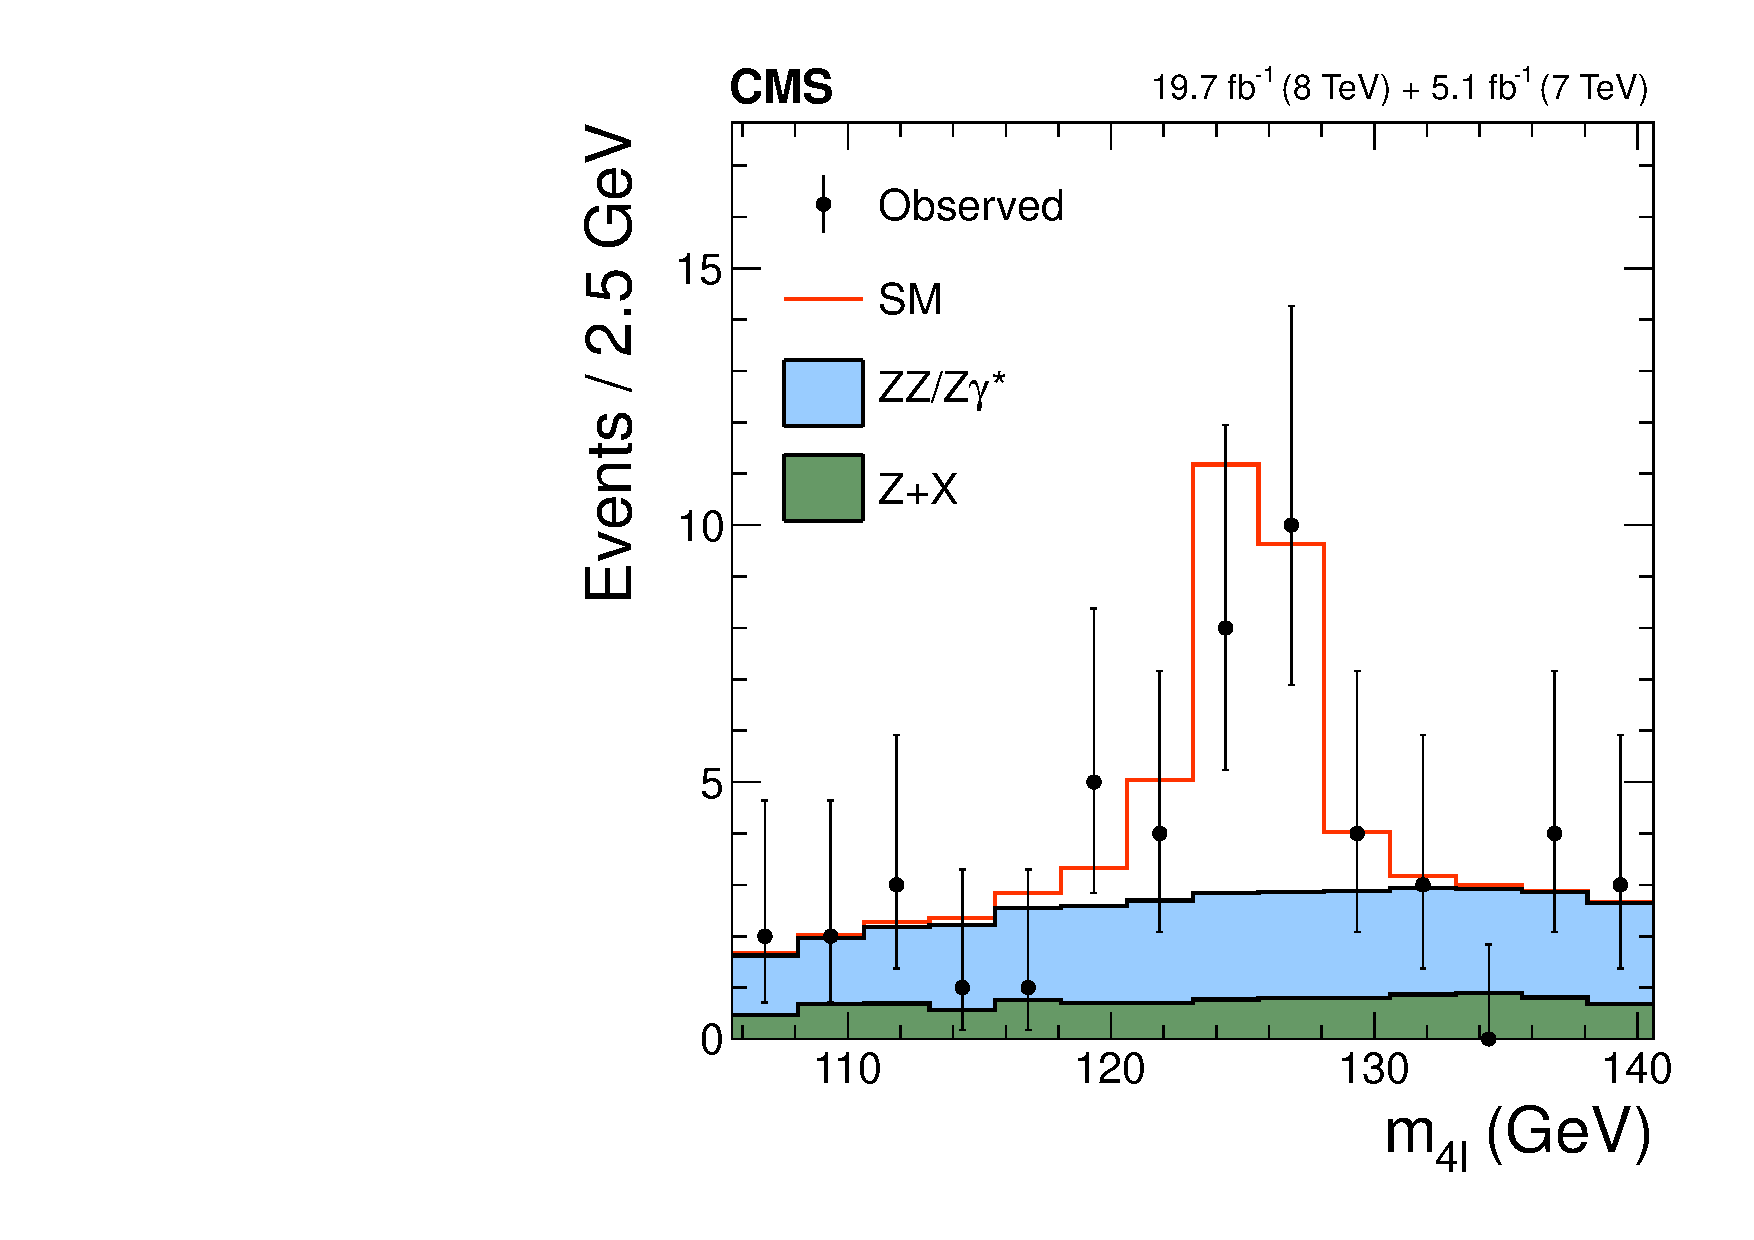
\includegraphics[width=0.50\linewidth]{figures/cCompare_DataMC_AllTeV_ZZMass.pdf}
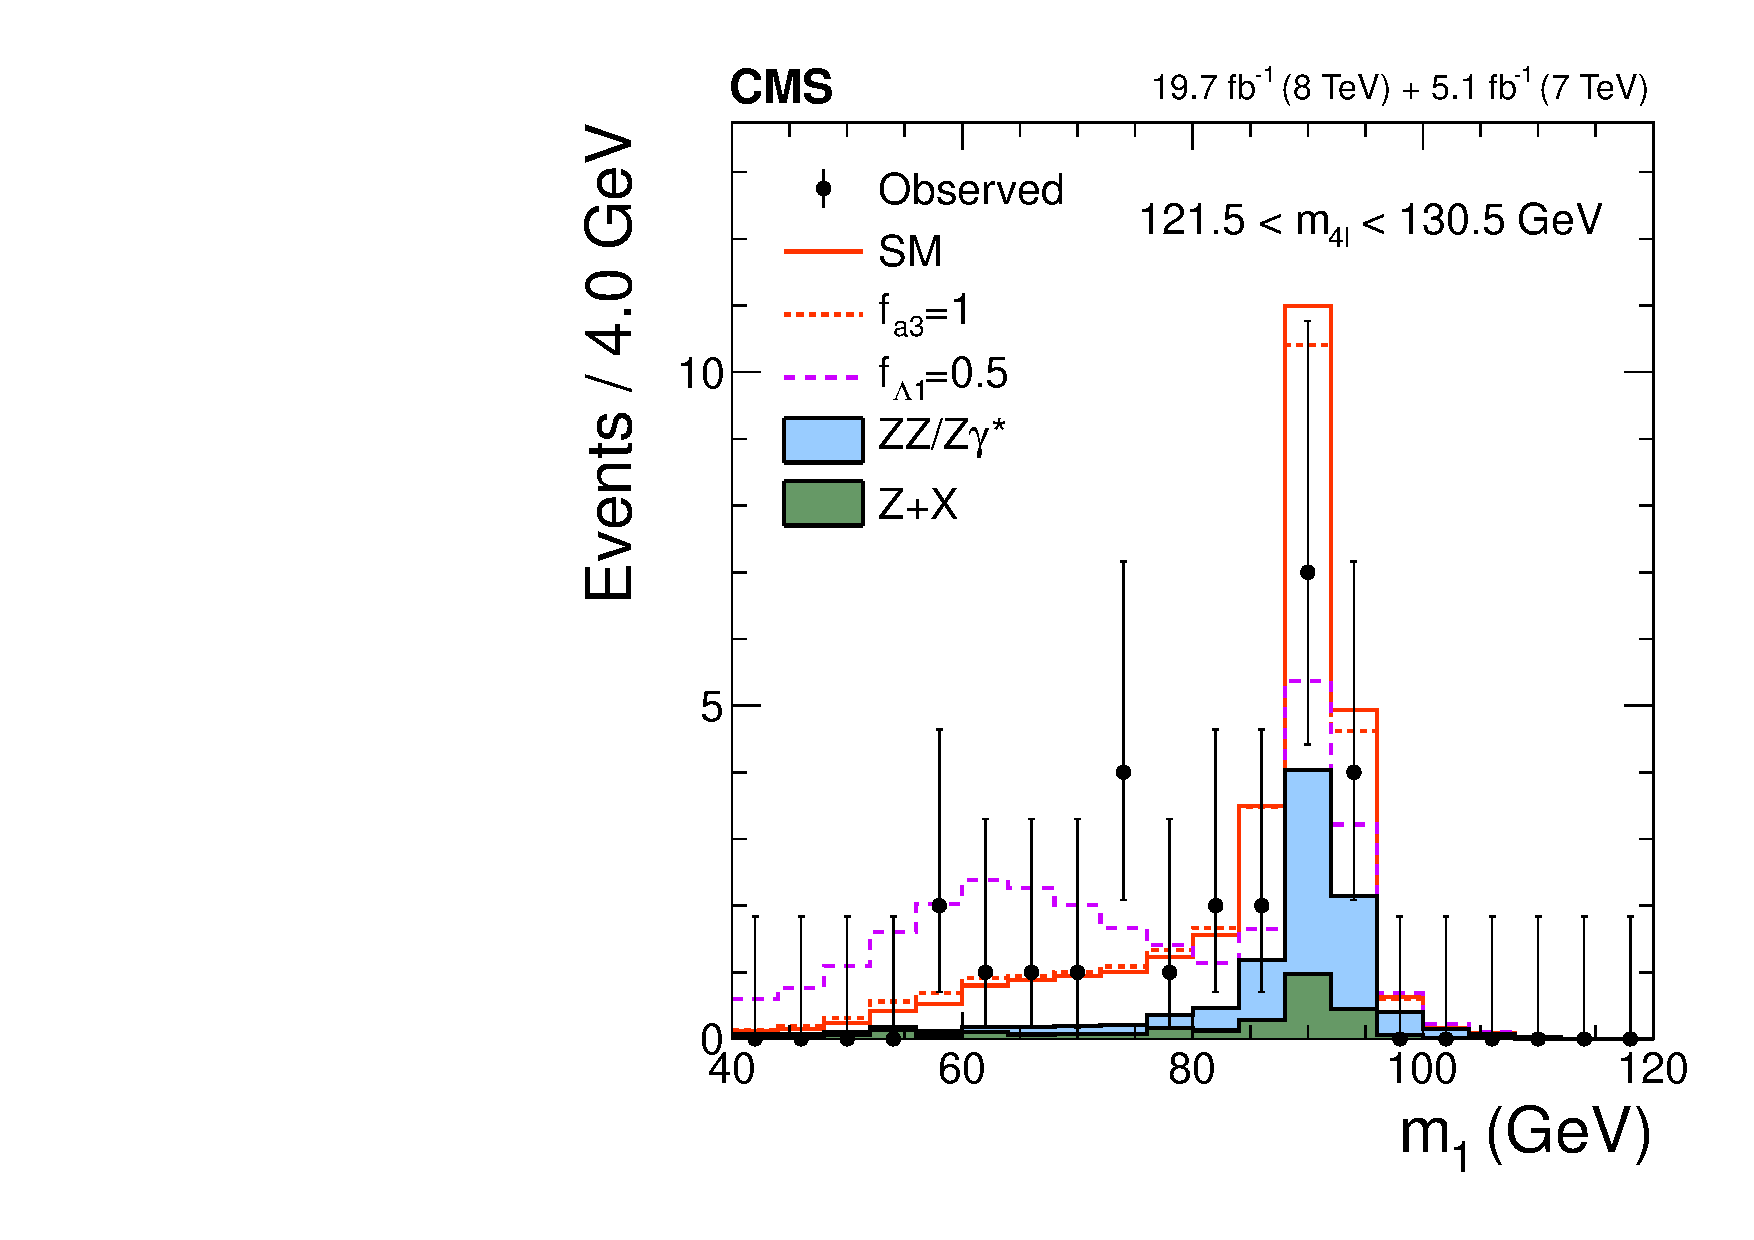
\includegraphics[width=0.50\linewidth]{figures/cCompare_DataMC_AllTeV_Z1Mass_SignalEnriched.pdf}
}
\caption{ Distributions of two out of the eight kinematic observables
  used in the $\chanHZZ$ analysis: $m_{4\ell}$, $m_1$.  Distributions
  show the observed data (points with error bars), the expectations
  for the SM background (shaded areas), the SM Higgs boson signal
  (open areas under the solid histogram), and the alternative
  spin-zero resonances (open areas under the dashed histograms).  The
  mass of the resonance is taken to be 125.6 GeV and the SM cross
  section is used.  The $m_1$ distribution is presented with the
  requirement $121.5 < m_{4\ell} < 130.5$ GeV.  
\label{fig:hzzkinematics} }
\end{center}
\end{figure}
%%%%%%%%%%%%%%%%%%%%%%%%%

One of the approaches pursued in this channels is to parameterise the
multidimensional distributions as a function of the parameters of
interests, which in this approach are the anomalous couplings. Given
the difficulty to populate eight-dimensional distributions for
components that cannot be described analytically, like the
$\Pg\Pg\to\PZ\PZ/\PZ\Pgs$ and $Z+$X processes, this approach is only
pursued for some of the measurements for a spin-zero resonance.
The analytic parameterization is the product of the differential decay cross section, 
$d\sigma_{4\ell}$, and the production spectrum, $W_{\mathrm{prod}}$, written as
%
\begin{eqnarray}
\label{eqn:gen_pdf}
{\cal P}(\vec{p}_\mathrm{T},Y,\Phi^*, \vec{x} | \vec{\zeta}) =
W_{\mathrm{prod}}(\vec{p}_\mathrm{T},Y,\Phi^*,\hat{s}) \times \\ \nonumber
\frac{d\sigma_{4\ell}(m_{4\ell},m_1, m_2, \vec\Omega | \vec{\zeta})}{dm_1^2dm_2^2d\vec\Omega}\,, 
\end{eqnarray}
%
where $\vec{p}_\mathrm{T}$, $Y$, and $\Phi^*$ are the transverse
momentum, rapidity, and azimuthal orientation of the four-lepton
system, and $\hat{s}=m_{4\ell}^2$ is the center-of-mass energy of the
parton-parton system. This probability is converted into
detector-level observables through transfer functions,
$T({\vec{x}^{\prime\mathrm{R}}} | \vec{x}^{\prime\mathrm{G}})$,
describing the detector response to produced leptons. Due to the
excellent angular resolution of the CMS tracker, the effect of the
resolution on the lepton direction is neglected.


The eight-dimensional analysis can be reduced to a three-dimensional
one by storing the full kinematic information in a discriminant
designed for the separation of either background (${\cal D}_{\rm
  bkg}$), the alternative signal components (${\cal D}_{J^P}$), or
interference between those components (${\cal D}_{\rm int}$).  The
construction of the kinematic discriminants follows the matrix element
likelihood approach ({\sc MELA}
package~\cite{Chatrchyan:2012ufa,Gao:2010qx,Bolognesi:2012mm,Anderson:2013afp}),
where the probabilities for an event are calculated using the LO
matrix elements as a function of angular and mass observables.  The
$\JHUGEN$ matrix elements are used for the signal, $\Pg\Pg$ or
$\qqbar\to \X\to \PZ\PZ$ / $\PZ\Pgs$ / $\Pgs\Pgs\to4\ell$, and $\MCFM$
matrix elements for the background, $\Pg\Pg$ or $\qqbar\to\PZ\PZ$ /
$\PZ\Pgs$ / $\Pgs\Pgs$ / $\PZ\to 4\ell$.
%
To remove the dependence of the spin-one and spin-two discriminants on
the production model, the probability ${\cal P}^{\rm kin}$ is averaged
over the two production angles $\cos\theta^*$ and $\Phi_1$, or
equivalently the signal matrix element squared is averaged over the
polarization of the resonance~\cite{Anderson:2013afp}, defining two
production-mechanism-independent discriminants, equivalent to the ones
for a spin-zero resonance: ${\cal D}^{\rm dec}_{\rm bkg}$ and ${\cal
  D}^{\rm dec}_{J^P}$.

\subsection{Kinematics of $\chanHWW$}
\label{sec:hwwkinematics}

For the $\chanHWW$ decay, events with exactly one electron and one
muon are selected, passing tight identification criteria to suppress
the reducible background from $\wjets$ processes, as described in
Ref.~~\cite{Chatrchyan:2013iaa}.  The events with two same-flavor
leptons are not considered for the high Drell-Yan background.  The
$\mathrm{e}\mu$ pair is required to have an invariant mass above
$12\GeV$, and a \pt above $30\GeV$. Events are also required to have
\textit{projected}~$\MET$ above 20~$\GeV$, as defined in
Ref.~\cite{Chatrchyan:2013iaa}. Signal events with exactly zero or one
jet reconstructed satisfying $\et>30~\GeV$ and $|\eta|<$~4.7 are
dominated by gluon fusion Higgs boson production, while events with
exactly two jets are dominated by VBF production.

The main backgrounds, the non-resonant $\PW\PW$ production and
top-quark production ($\ttbar$ and $\tw$ processes, are estimated from
data.  The reducible background arising from misidentified leptons
from $\wjets$ processes is estimated from a data control sample with
loosened lepton identification. The contribution from the $\wgamma^*$
process is also estimated from data with three leptons. The residual
minor backgrounds from triboson ($\V\V\V$) and sub-dominant $\PW\PZ$
and $\PZ\PZ$ are estimated from simulation.
%
The event yields observed in data and the expectation from 
the different processes are given in Ref.~\cite{Chatrchyan:2013iaa}.
%
As a difference with the $\chanHZZ$ case, only partial reconstruction
of the four leptons is possible in this channel, because of the two
undetected neutrinos. Two distributions are used in this case,
summarizing the kinematics of the two detected charged leptons and the
$\met$ of the event: the transverse mass of the final state ($\mth$),
defined as $\mth^2 = 2 \ptll \met (1-\cos\delphillmet)$, and the
dilepton mass ($\mll$) which is one of the most discriminating
kinematic variables for a Higgs boson with low mass, and it is also
correlated to the spin via the azimuthal opening angle between the
two leptons. 
%
The signal region is defined by $\mll < 200$~GeV, and $60 \leq \mth
\leq 280~\GeV$.  The distributions of these observables for data, an
expected SM Higgs signal and backgrounds are presented in
Fig.~\ref{fig:hwwkinematics} for events with no reconstructed jets,
which is the most sensitive category of this analysis.
%

%%%%%%%%%%%%%%%%%%%%%%%%%
\begin{figure}[!p]
\begin{center}
\centerline{
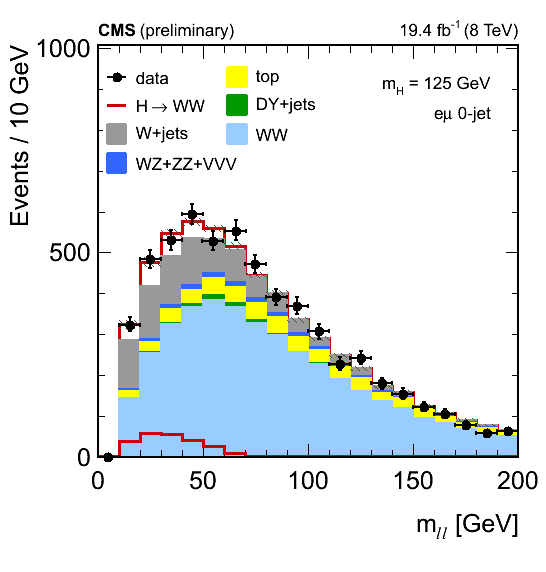
\includegraphics[width=0.50\linewidth]{figures/wwpresel_0j_mh125_massll.png}
~~~~~
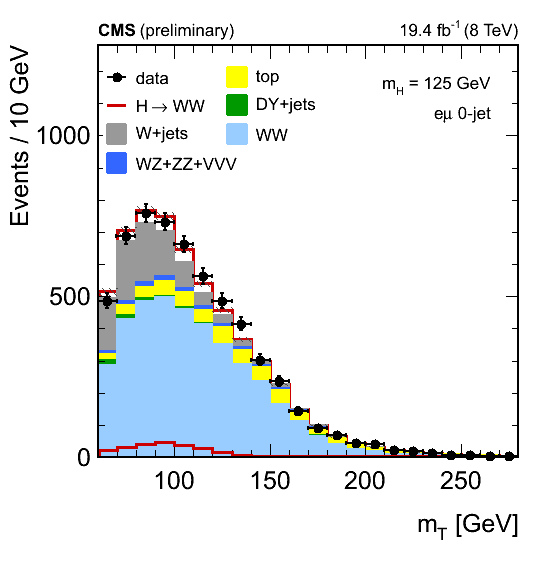
\includegraphics[width=0.50\linewidth]{figures/wwpresel_0j_mh125_mt.png}
}
\caption{ 
  Distributions of the two kinematic observables
  used in the $\chanHWW$ analysis: $\mll$, $\mth$.  Distributions
  show the observed data (points with error bars), the expectations
  for the SM background (filled areas), the SM Higgs boson signal
  (open areas on top of the solid histogram).  The
  mass of the resonance is taken to be 125 GeV and the SM cross
  section is used.  Events with zero jets are shown.  
\label{fig:hwwkinematics} }
\end{center}
\end{figure}
%%%%%%%%%%%%%%%%%%%%%%%%%


\subsection{Kinematics of $\chanHgg$}
\label{sec:hggkinematics}

For this decay channel, the kinematics of the di-photon events are
defined by the mesurement of the photon energy and position in the
ECAL. The selection for the spin-parity analysis is described in
Ref.~\cite{Khachatryan:2014ira}. The cosine of the scattering angle in
the Collins--Soper frame, $\cos\theta^*$, is used to discriminate
between the spin hypotheses.  The angle is defined in the diphoton
rest frame as that between the collinear photons and the line that
bisects the acute angle between the colliding protons:
%
\begin{equation}
  \costhetastar=2\times\frac{E^{\gamma2}p^{\gamma1}_{z}-E^{\gamma1}p^{\gamma2}_{z}}{\mgg\sqrt{\mgg^{2}+(\ptgg)^{2}}},
\end{equation}
%
where $E^{\gamma1}$ and $E^{\gamma2}$ are the energies of the leading
and subleading photons, $p^{\gamma1}_{z}$ and $p^{\gamma2}_{z}$ are
the $z$ components of their momenta, and $\mgg$ and $\ptgg$ are the
invariant mass and transverse momentum of the diphoton system.  In the
rest frame of a spin-0 boson the decay photons are isotropic, and so,
before the acceptance requirements, the distribution of \costhetastar
is uniformly flat under the SM hypothesis.  In general this is not
the case for the decay of a spin-2 particle.  Within each diphoton
class, the events are categorized in five $|\cos\theta^*|$ bins to
discriminate between the different spin hypotheses, and in several
$(\eta, R_9)$ categories to enhance the sensitivity.
%



\section{Study of exotic spin-one and spin-two couplings}
\label{sec:exotics}
\subsection{$\PH\to\V\V\to4\ell$ final states}
\label{sec:exotic_h4l}

With the $\chanHZZ$ and $\chanHWW$ decay channels the exotic-spin
$J^P$ hypotheses for the 125 $\GeV$ resonance are tested again the SM
one. In addition, mixed spin-one state hypotheses, as well as the
comprehensive set of spin-two models listed in
Sec.~\ref{sec:phenomenology} are tested. Finally, the fractional
presence of $J^P$ models of a state nearly degenerate in mass with the
SM state are tested.

For these studies, template maximum likelihood fits to the kinematic
discriminants defined in Sec.~\ref{sec:hzzkinematics} are used.  In
the case of $\chanHZZ$ and spin-one, they are
$(\superKD,\psvectorKD,\vectorKD)$. These hypotheses are tested for a
discrete set of values for parameter $f_{b2}$ both for $\qqbar$
production and for generic production, using production-independent
discriminants. All spin-one tests are consistent with the expectation
for the SM Higgs boson.  While the decay-only analysis uses less
information and is expected to provide weaker constraints, the
fluctuations in the observed data lead to stronger constraints for
spin-one models.  The least restrictive result corresponds to the
$1^+$ model in the $\qqbar$ production test with a CL$_s$ value of
$0.031\%$. Any arbitrary spin-one model for the resonance observed in
the $\X\to \PZ\PZ\to 4\ell$ decay mode with any mixture of parity-even
and parity-odd interactions and any production mechanism is excluded
at a CL of 99.97\% or higher. A summary is shown in
Fig.~\ref{fig:jp_summary_1} (left).

In the case of $\chanHWW$ The average separation between the SM Higgs
boson and each alternative spin-1 hypothesis is larger than one
standard deviation. The alternative spin-1 hypotheses are disfavored
with CLs values of 3.9\% for $1^-$, 14.0\% for $1^{+}$, and 8.7\% for
$1_{mix}$. The distribution of the test statistic and the observed
value for the case of $1^-$ against SM is shown in
Fig.~\ref{fig:jp_summary_1} (right).



%%%%%%%%%%%%%%%%%%%%%%%
\begin{figure}[!htbp]
  \begin{center}
\centerline{
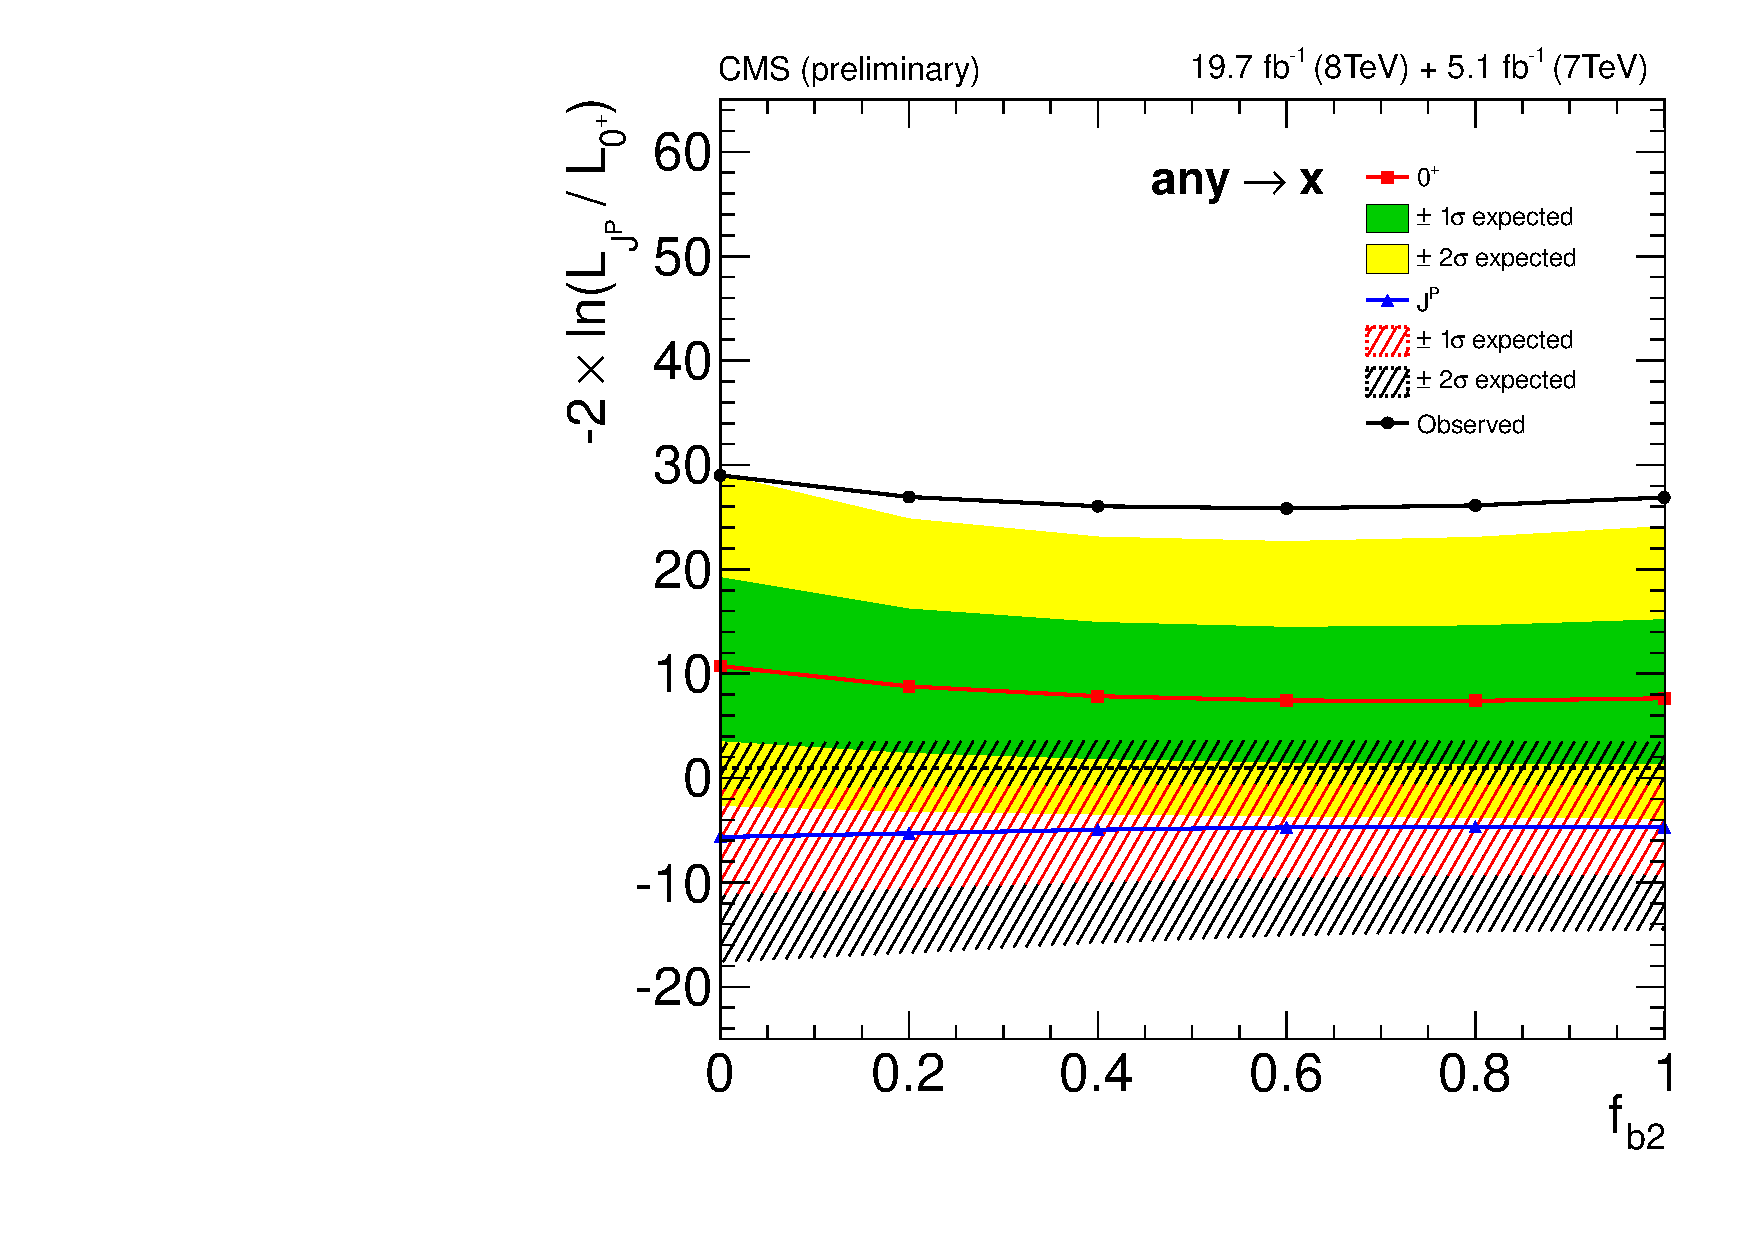
\includegraphics[width=0.50\linewidth]{figures/hzz_spin1_summary_PI.pdf}
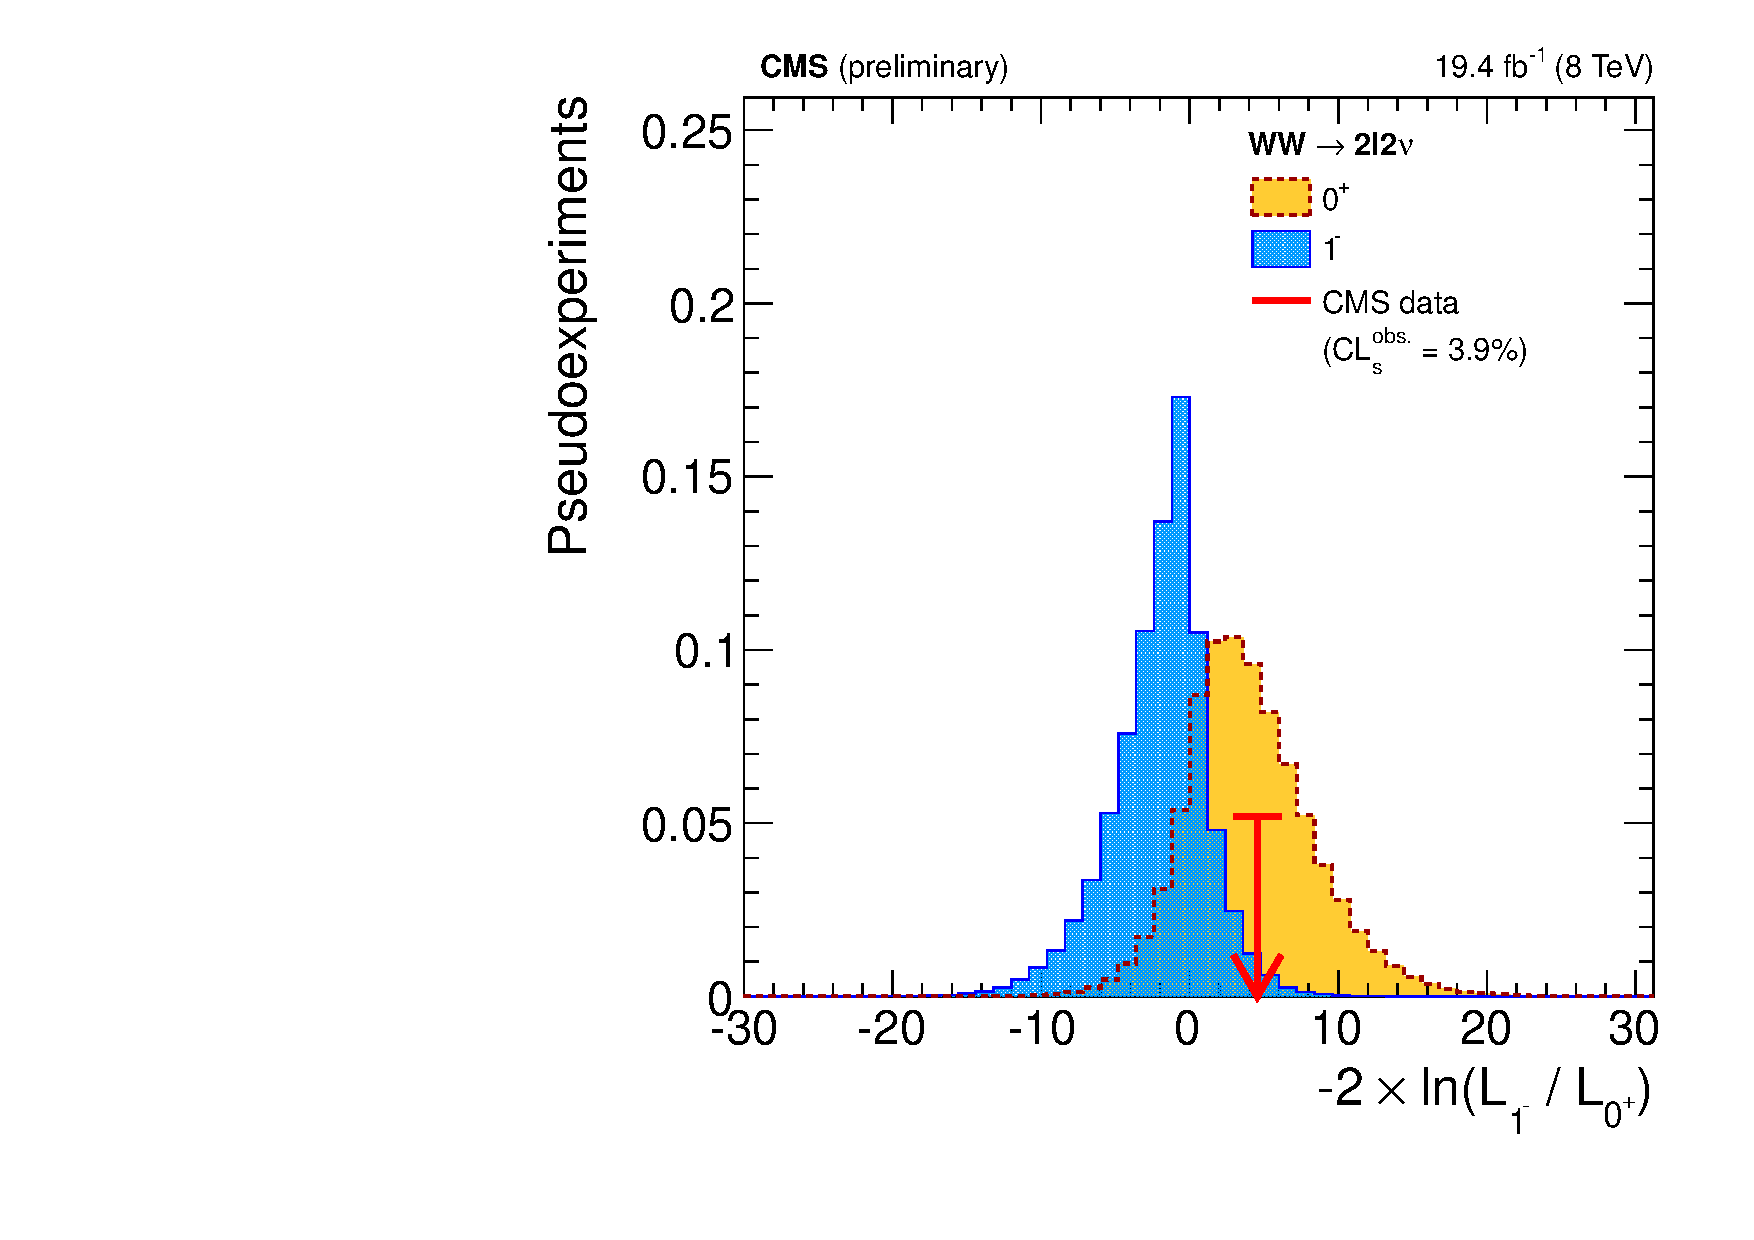
\includegraphics[width=0.50\linewidth]{figures/hzww_spin1_q1minus.pdf}
}
\caption{Left: the expected and observed distributions of median
  test-statistic $q$ for alternative mixed spin-one hypotheses, as
  a function of $f_{b2}$, for $\chanHZZ$, production-independent
  test.  The green and yellow filled bands represent the 1$\sigma$
  and 2$\sigma$ around the median expected value for the SM Higgs
  boson hypothesis. The red and black dashed bands represent the
  1$\sigma$ and 2$\sigma$ around the median expected value for the
  mixed spin-one hypotheses.  Right: Distributions of $-2
  ln(L_{1^-} /L_{0^{+}_{m}})$, combining the 0-jet and 1-jet
  categories, for the $\chanHWW$, channel with $\qqbar$
  production, pure $1^-$ state. The observed value is indicated by
  the red arrow.
  \label{fig:jp_summary_1}} 
  \end{center}
\end{figure}
%%%%%%%%%%%%%%%%%%%%%%%

The hypothesis test of SM Higgs boson against the spin-two resonance
is performed for ten models and three scenarios: $\Pg\Pg$, $\qqbar$
production, and using only decay information in the $\chanHZZ$ decay
channel. Interference between the different amplitude components is
not considered in this case The data disfavor all tested spin-two
hypotheses in favor of the SM hypothesis $0^+$ with $1-$CL$_s$ values
larger than 99\% CL in the case of analysis of decay-only observables.
There are non-zero correlations between the best-fit values obtained
for the various alternate hypotheses.  All results are consistent with
the SM expectation. Measurements are also performed for two
non-interfering states, indicating no evidence for the presence of a BSM
one. Fig.~\ref{fig:jp_summary_2} (left) shows the distribution of the test 
statistic $q$ for one of these tests ($2_{h2}^+$).

%%%%%%%%%%%%%%%%%%%%%%%
\begin{figure}[!htbp]
\begin{center}
\centerline{
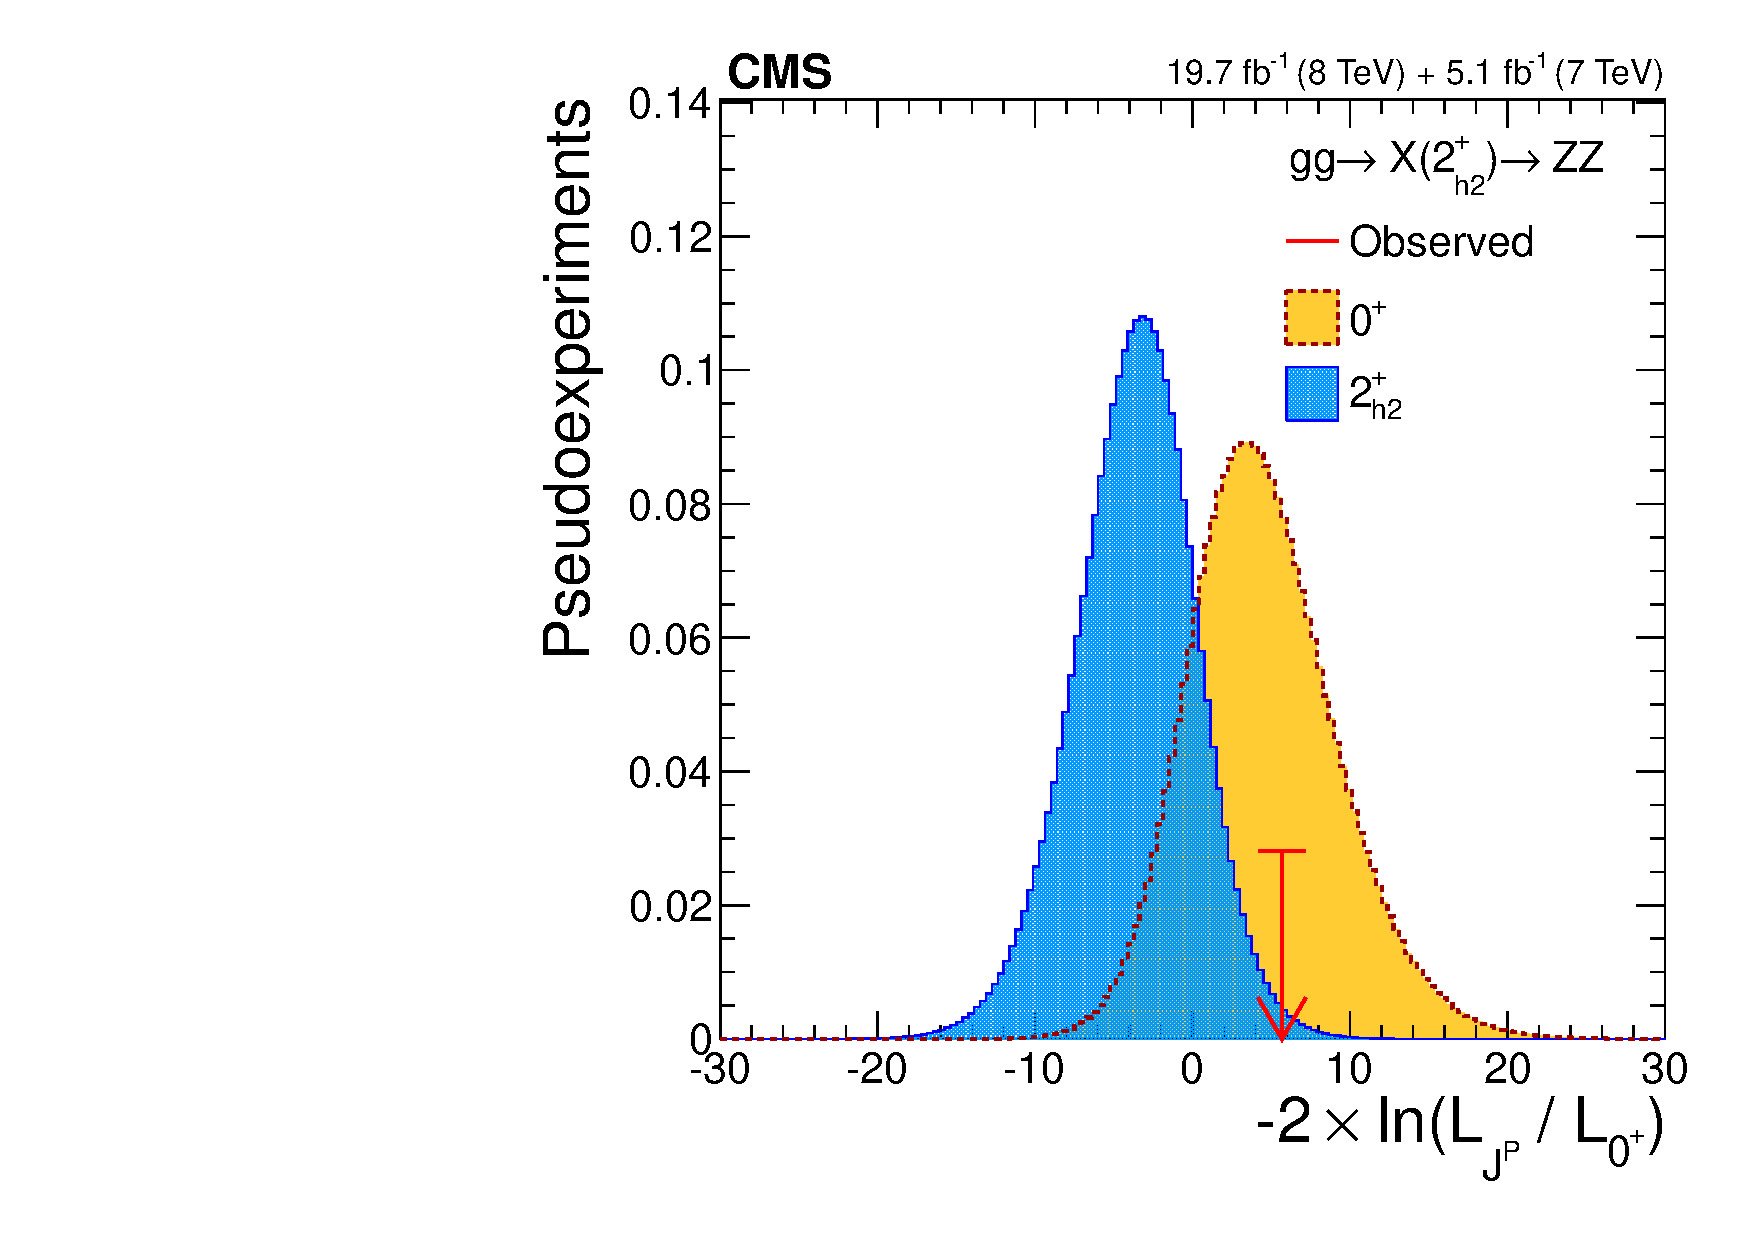
\includegraphics[width=0.45\linewidth]{figures/hzz_sigsep_combine_gg_2h2+.pdf}
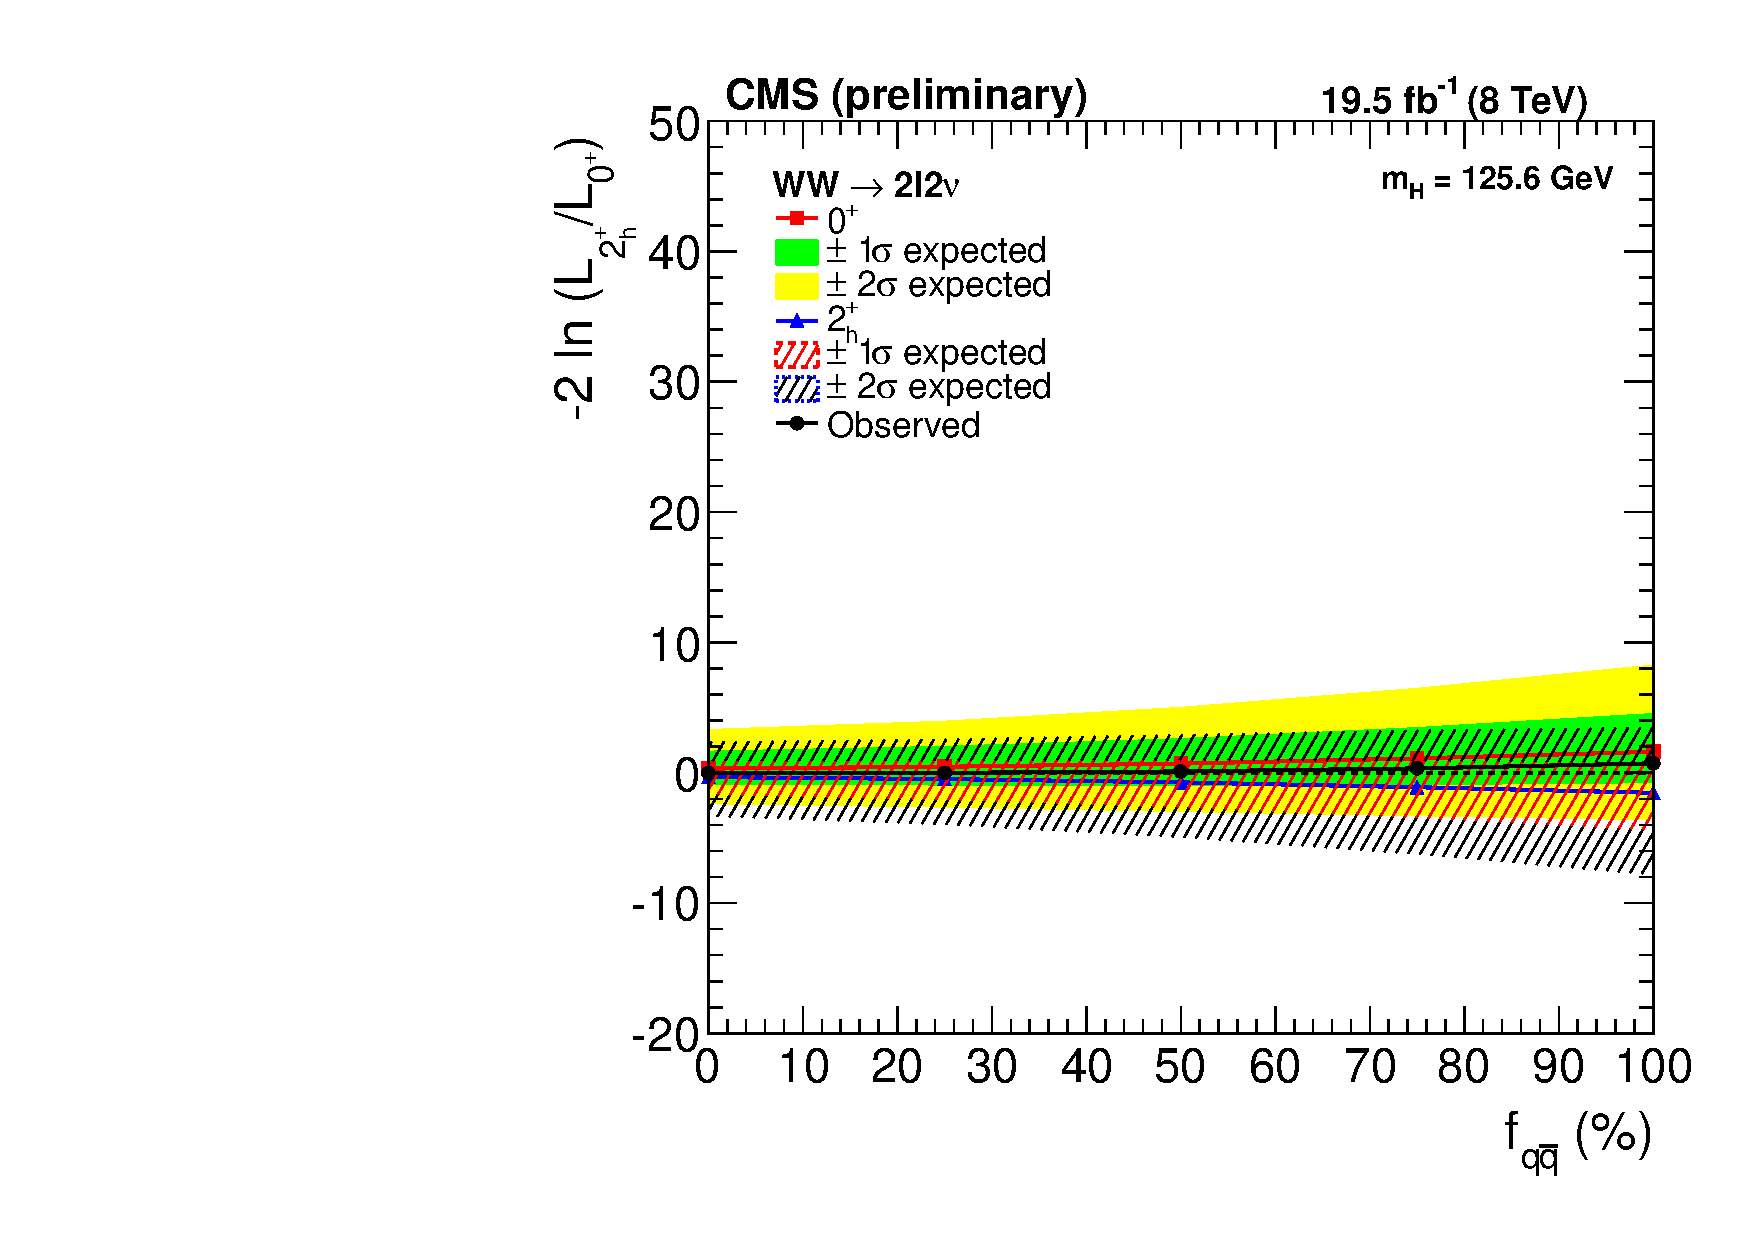
\includegraphics[width=0.45\linewidth]{figures/hww_sigsep_combine_2h2+.pdf}
}
\caption{ Left: Distributions of the test statistic $q=-2\ln({\cal L}_{J^P}/{\cal L}_{0^+})$ 
       for the $J^P=2^+_{h2}$ hypothesis of $\Pg\Pg\to\X(2^+_{h2})\to \PZ\PZ$
      tested against the SM Higgs boson hypothesis ($0^+$). 
            The expectation for the SM Higgs boson is represented by the yellow histogram on the right and the alternative $J^P$ hypothesis by the
      blue histogram on the left. The red arrow indicates the observed $q$ value.  
      Right: Observed and expected median test statistic for the $0^+$ and $\mathrm{J}=2$ hypotheses, as a function of the $f_{q\bar{q}}$ fraction for
      the $J^P=2^+_{h2}$ in the $\chanHWW$ decay mode.
\label{fig:jp_summary_2}}
\end{center}
\end{figure}
%%%%%%%%%%%%%%%%%%%%%%%


The results of the hypothesis testing for the spin-one and spin-two
hypotheses obtained by considering the $\X\to\PZ\PZ\to4\ell$ and
$\X\to\PW\PW\to\ell\nu\ell\nu$ decay channels can be combined, with the
assumption that the same tensor structure for the interactions appears
in both $\X\PZ\PZ$ and $\X\PW\PW$ couplings.  In case of the spin-one
studies, we have tested the models in which the new boson is produced
in the $\qqbar$ process. In case of the spin-two studies, we have
tested the models in which the new boson is allowed to be produced in
both the $\Pg\Pg$ and $\qqbar$ processes.  We have performed these
tests for several choices of the ratio of the two production rates
$f_{\qqbar}$.  The analysis which uses information from the $\chanHZZ$
decay channel is performed in an production-independent way.  Part of
the analysis which is based on the $\chanHWW$ decay channel tests for
several choices of the ratio of the $f_{\qqbar}$ ratio explicitly.
The expected separations from the test statistic distributions for all
the considered models are summarized in 
Figure~\ref{fig:jp_summary_comb}. The data disfavour all tested
spin-one and spin-two hypotheses in favour of SM hypothesis $0^+$ with
CL$_s$ value larger then 99.9\% CL. Each of these exclusions is tested
and reported independently of the other hypotheses, but one should
note that there are correlations between the various alternate
hypotheses.

%%%%%%%%%%%%%%%%%%%%%%%
\begin{figure}[!htbp]
  \begin{center}
    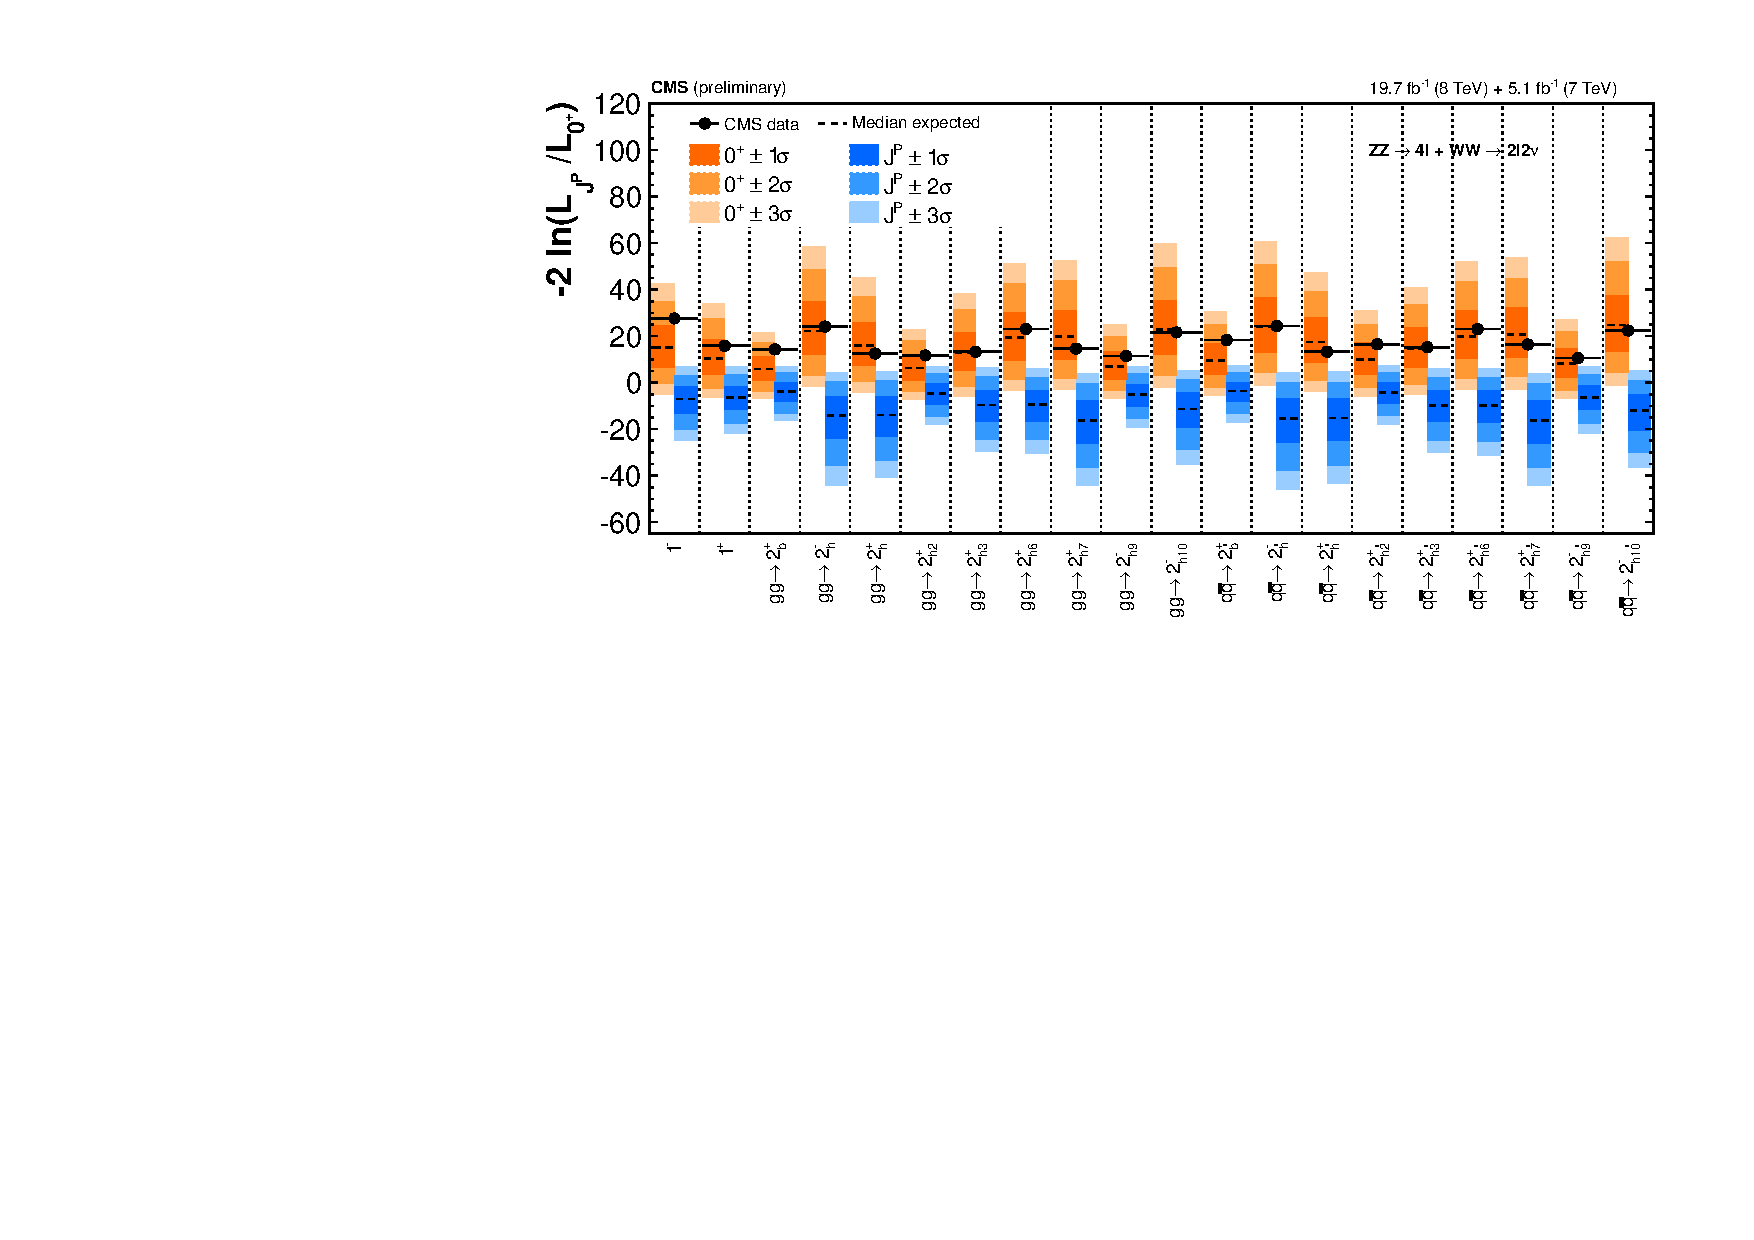
\includegraphics[width=0.95\linewidth]{figures/JP_SummaryPlot.pdf}
    \caption{
     Summary of the expected and observed values for the
      test-statistic $q$ distributions for the alternative spin-one and spin-two
      hypotheses tested with respect to the SM Higgs boson, based on the 
     combined analysis in $\chanHZZ$ and 
     $\chanHZZ$ decay channels.  The
      orange (blue) bands represent the 1$\sigma$, 2$\sigma$, and
      3$\sigma$ around the median expected value for the SM Higgs
      boson hypothesis (alternative hypothesis). The black point
      represents the observed value.
      \label{fig:jp_summary_comb}} 
  \end{center}
\end{figure}
%%%%%%%%%%%%%%%%%%%%%%%


\subsection{$\PH\to\Pgg\Pgg$ final state}
\label{sec:exotic_hgg}

Figure~\ref{fig:hgg_spin2} (left) shows the distribution of the
expected signal strength, $\mu$, relative to the SM expectation in the
five bins of $\abscostheta$ for the SM, and for two $2_m^+$ models:
where the $2_m^+$ resonance is produced entirely by gluon-fusion
($\Pg\Pg$), and where it is produced entirely by quark-antiquark
annihilation ($\Pq\Paq$).  The hypothesis of SM Higgs boson is
tested against two alternative models of a $2_m^+$ resonance produced
entirely by either gluon-fusion, or entirely by quark-antiquark
annihilation, or by three intermediate mixtures of $\Pg\Pg$ and
$\Pq\Paq$ spin-2 production, with a fraction of cross section
$f_{\qqbar}$. Figure~\ref{fig:hgg_spin2} (right) shows the values of
the test statistic as a function of $f_{\qqbar}$.  The hypothesis of the
signal being $2_m^+$ is disfavoured for all values of $f_{\qqbar}$
tested.


\begin{figure}[!hbtp]
  \begin{center}
    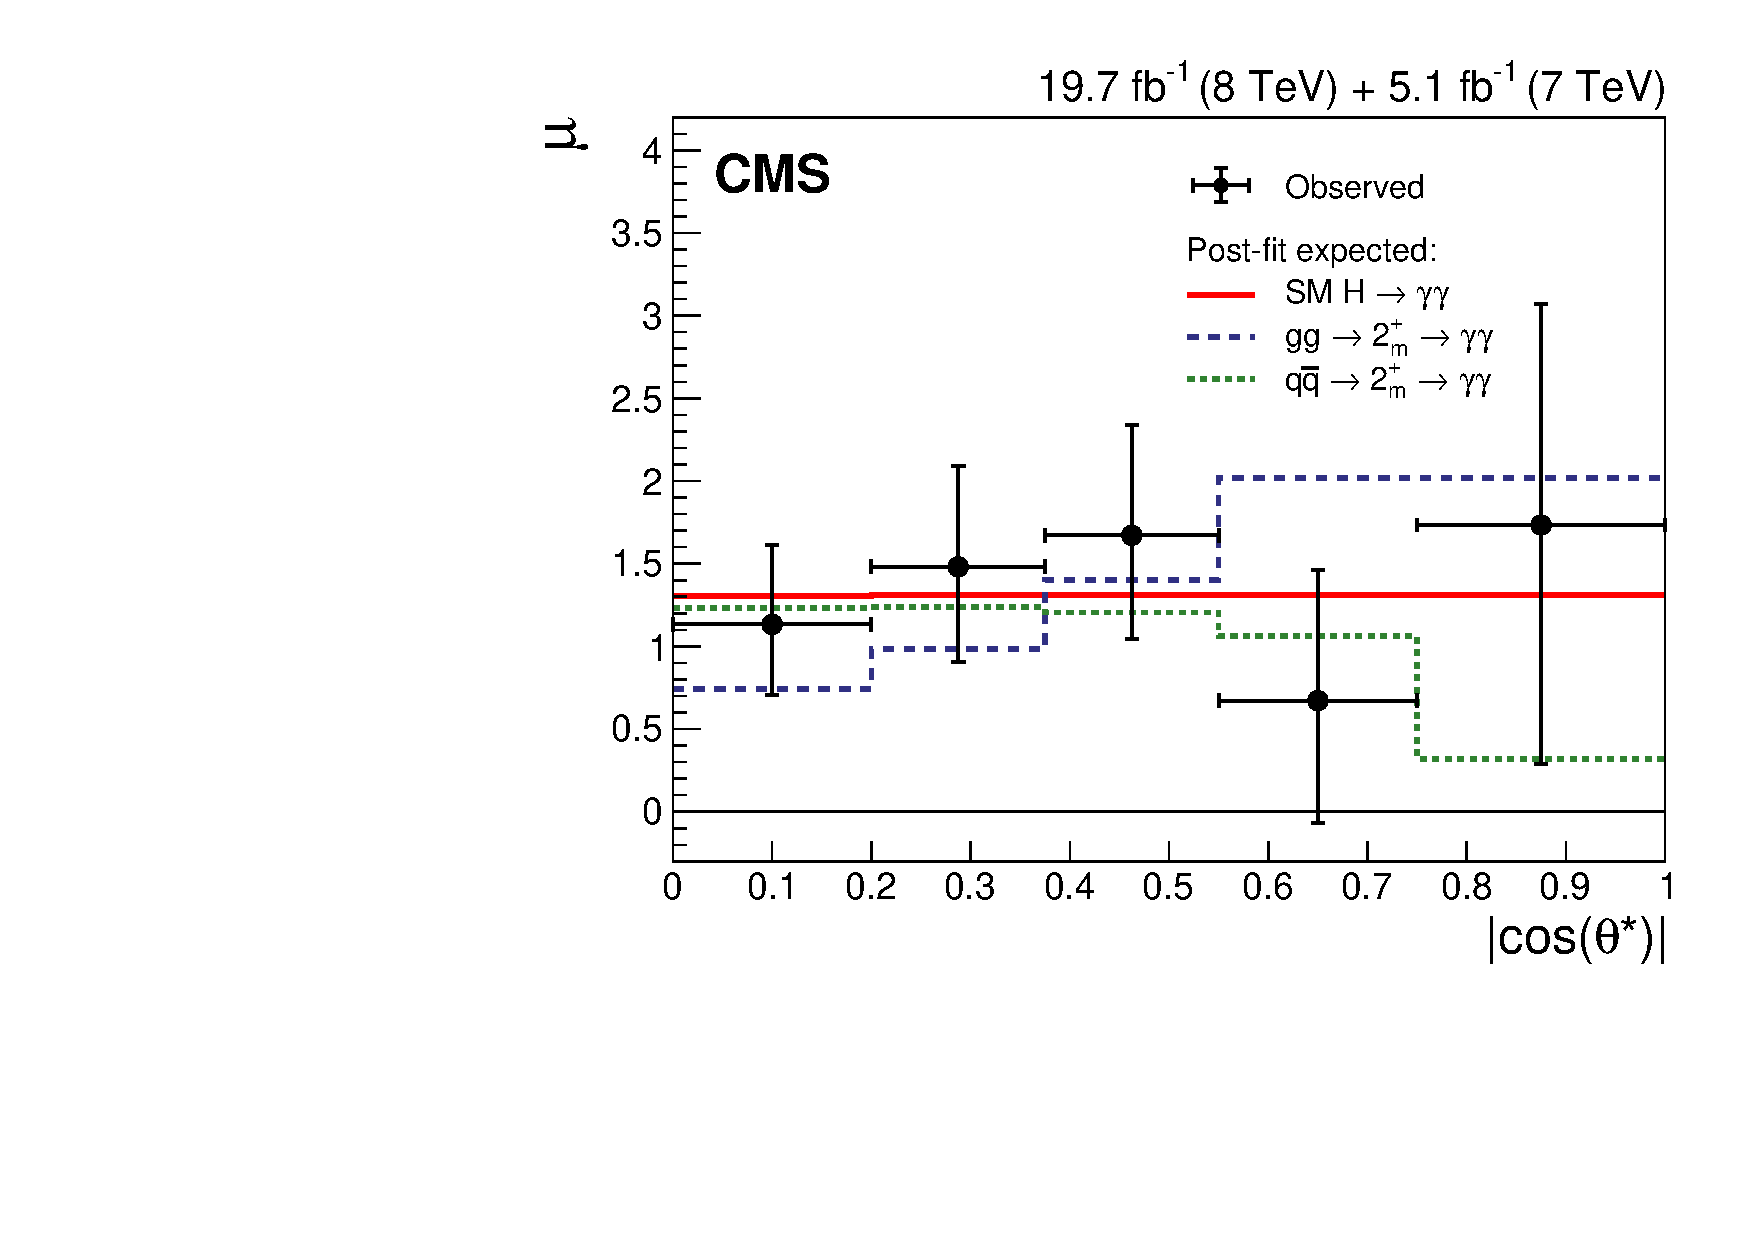
\includegraphics[width=0.49\linewidth]{figures/hgg_mucosth.pdf}
    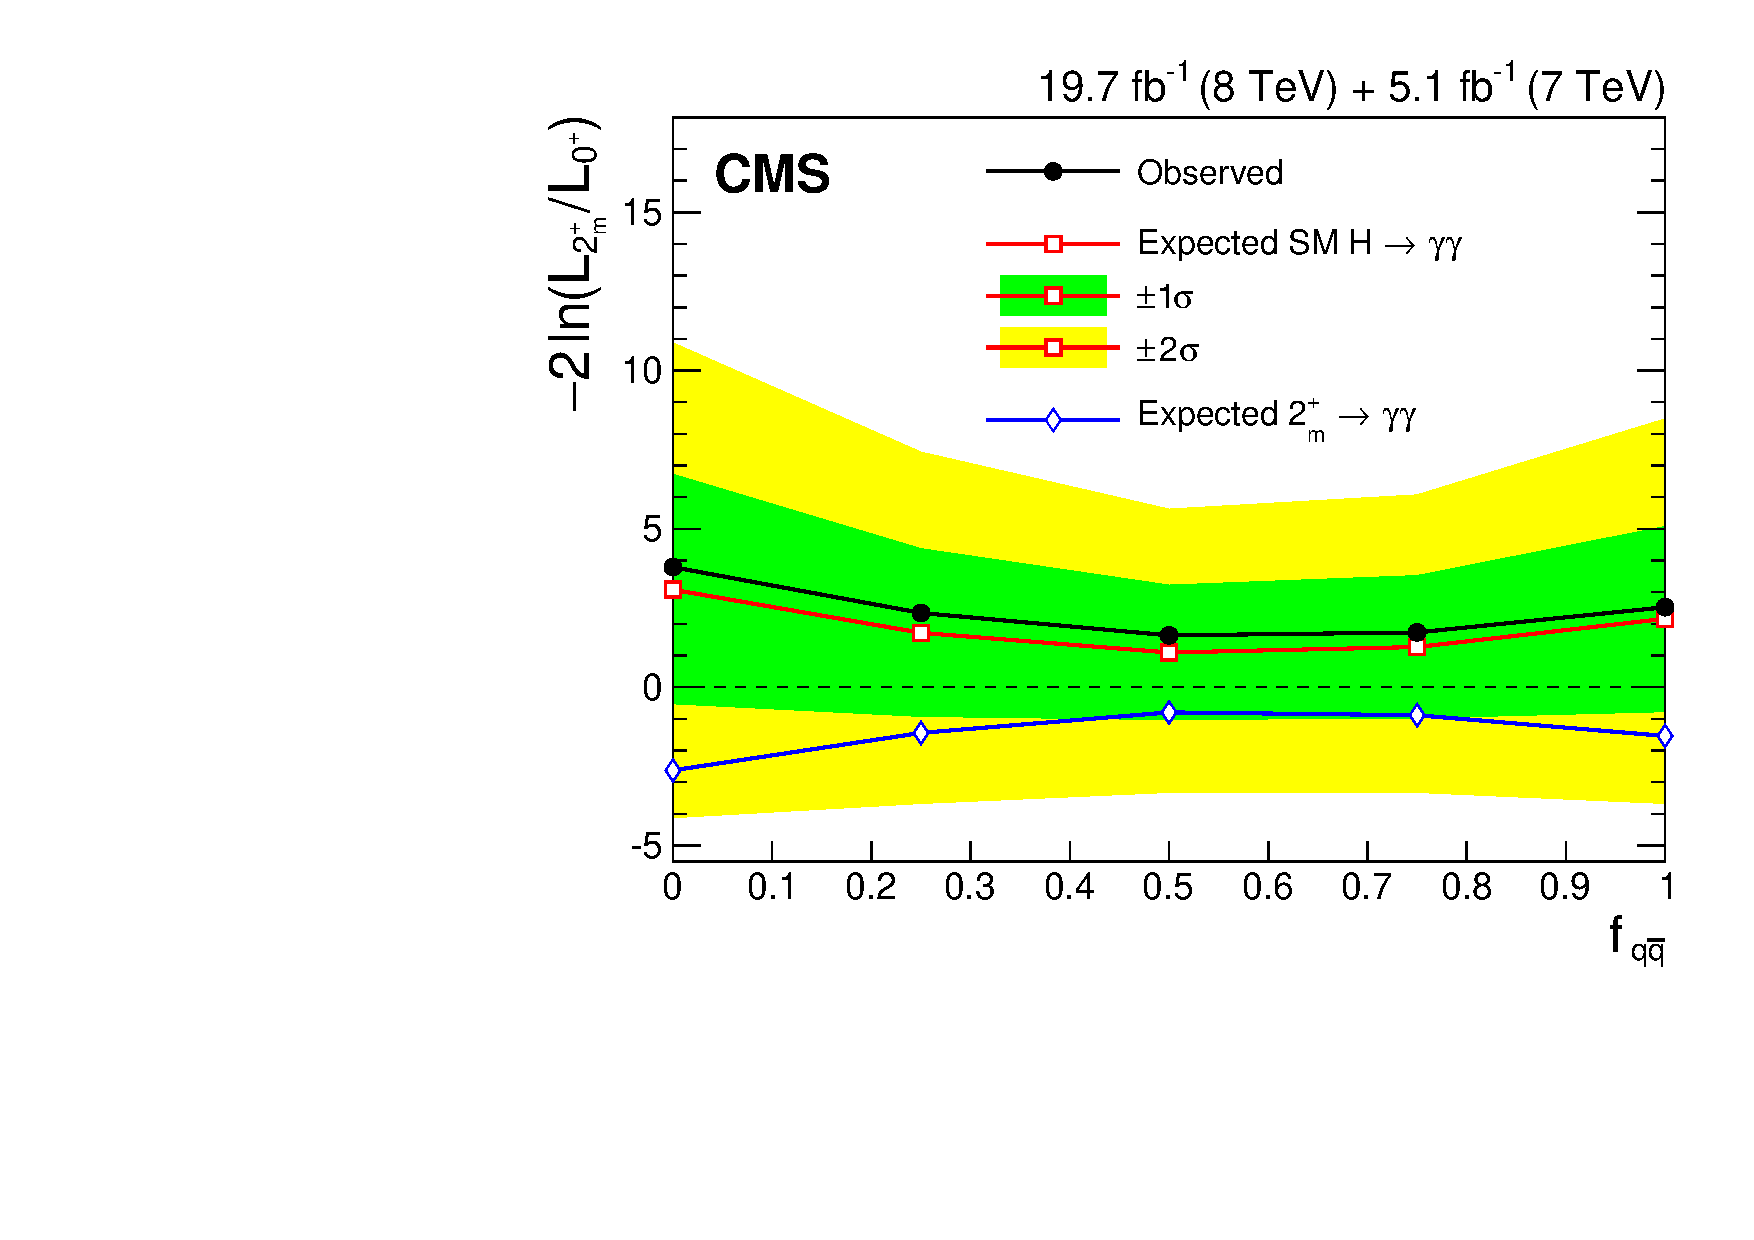
\includegraphics[width=0.49\linewidth]{figures/hgg_spin2_excl.pdf}
    \caption{Top: Signal strength in five bins of $\abscostheta$ expected for SM, for $2^+_m$ produced
      by $\Pg\Pg$, and for $2^+_m$ produced by $\qqbar$.
      The signal strength observed in the data is shown by the black points.
      Right: Test statistic for pseudo-experiments generated under the SM hypothesis (open squares) and the
$2^+_m$, hypothesis (open diamonds), as a function of the $f_{\qqbar}$ fraction.
      The observed distribution in the data is shown by the black points.
      \label{fig:hgg_spin2}
    }
  \end{center}
\end{figure}





\section{Study of spin-zero HVV couplings}
\label{sec:spinzero}
Since an extensive set of exotic resonances have been excluded,
measurements are presented of the anomalous coupling for a spin-zero
boson decaying into two EW massive gauge bosons ($\PZ\PZ$ or
$\PW\PW$).
%
The analysis consider three sets of measurements:
%
\begin{enumerate}
\item Constraints on the presence of only one anomalous term in the
  $\PH\V\V$ amplitude of Eq.~(\ref{eq:formfact-fullampl-spin0}), where
  the couplings are considered to be real, i.e. $\phi_{ai}=0$ or
  $\pi$, where $\phi_{ai}$ generically refers to the phase of the
  coupling in question, such as $\phi_{\Lambda1}$, $\phi_{a2}$, or
  $\phi_{a3}$. 
  %% The results of the likelihood function scan for the
  %% three parameters, $f_{ai}\cos\phi_{ai}$, are shown in
  %% Fig.~\ref{fig:results_ZZ_1D}, where the $\cos\phi_{ai}$ term
  %% allows for a signed quantity with $\cos\phi_{ai}=-1$ or $+1$. 
  These measurements show no evidence of anomalous couplings.  The
  measurement of the same quantities can be also performed by allowing
  the coupling to be generically complex, by leaving its phase
  completely unconstrained. Also these measurement, though with
  smaller sensitivity, show consistency with the SM expectation. 

  
%%%%%%%%%%%%%%%%%%%%%%%%%
%% \begin{figure}[!p]
%% \begin{center}
%%        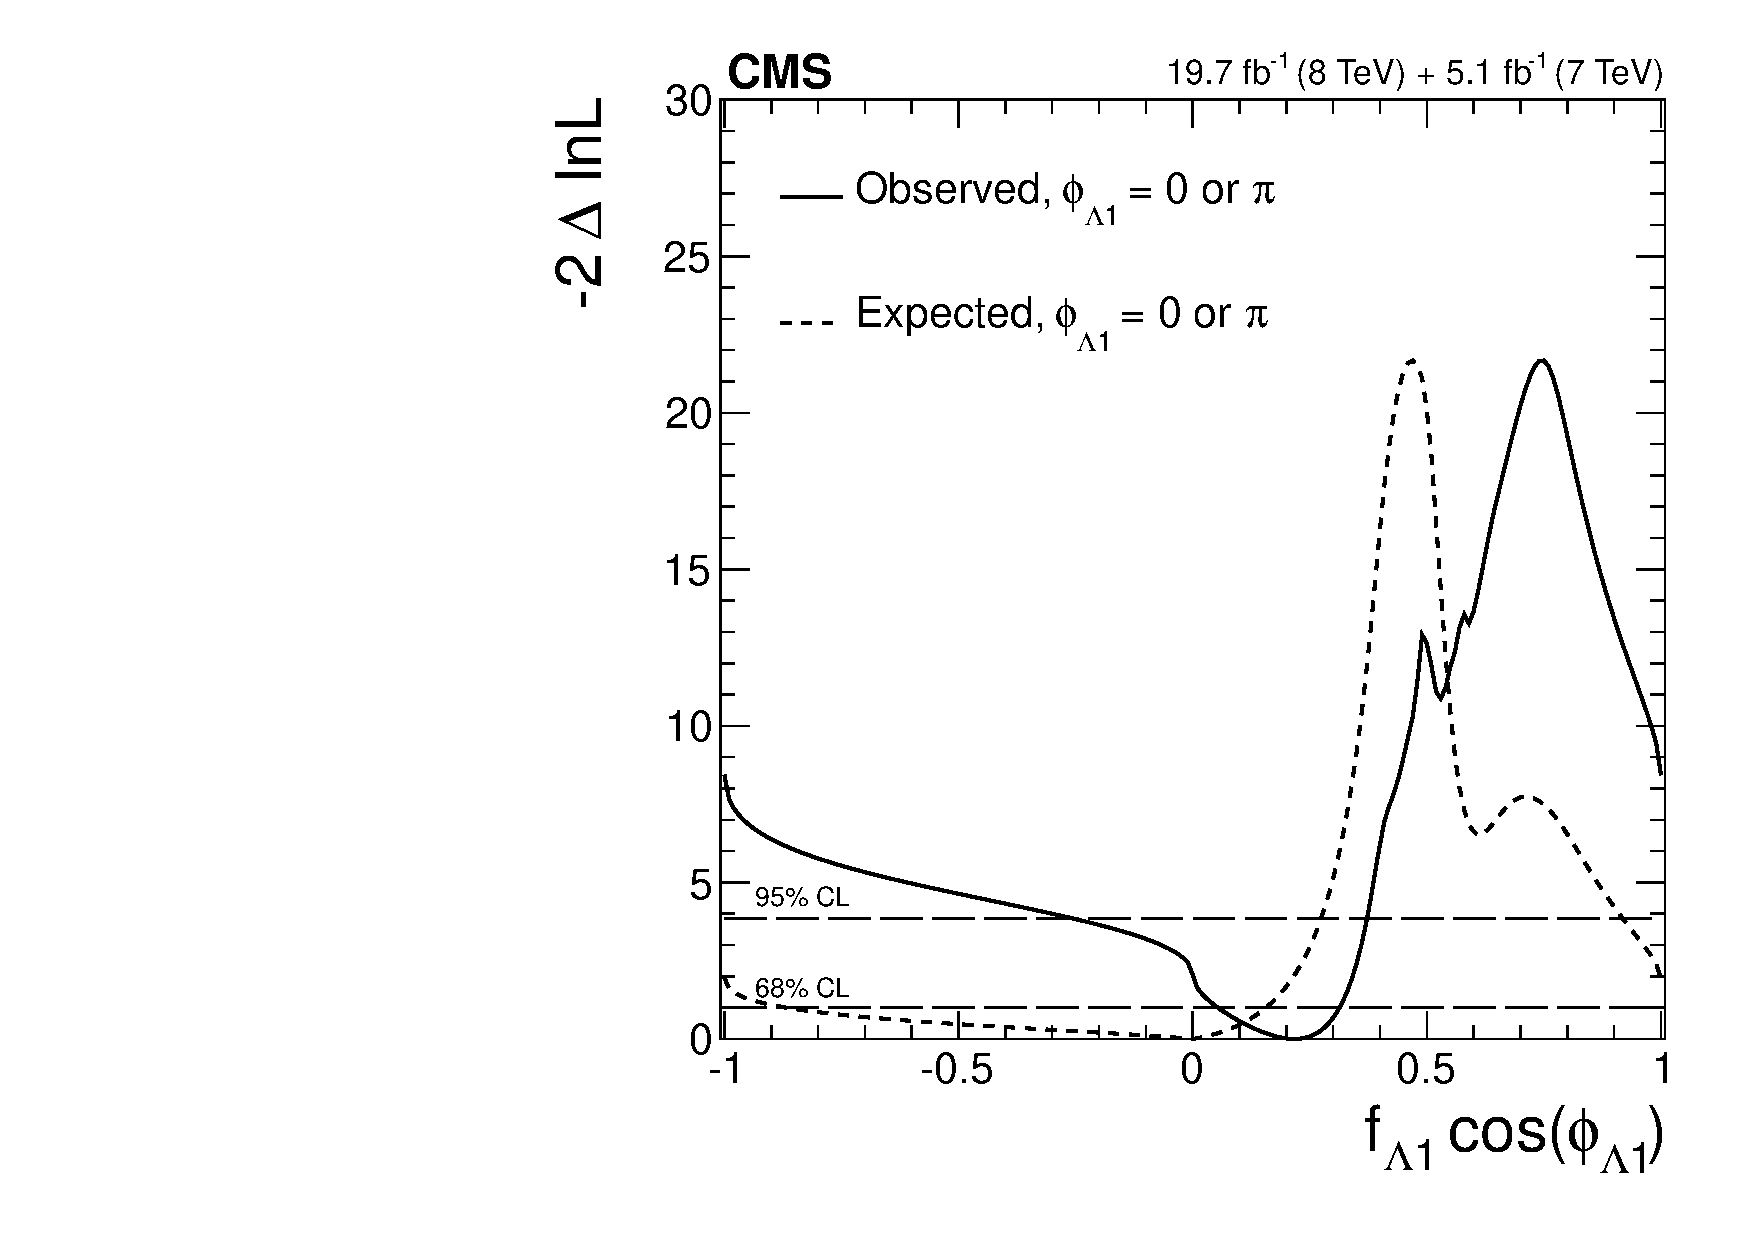
\includegraphics[width=0.31\linewidth,angle=0]{figures/fL1_Real.pdf}
%%        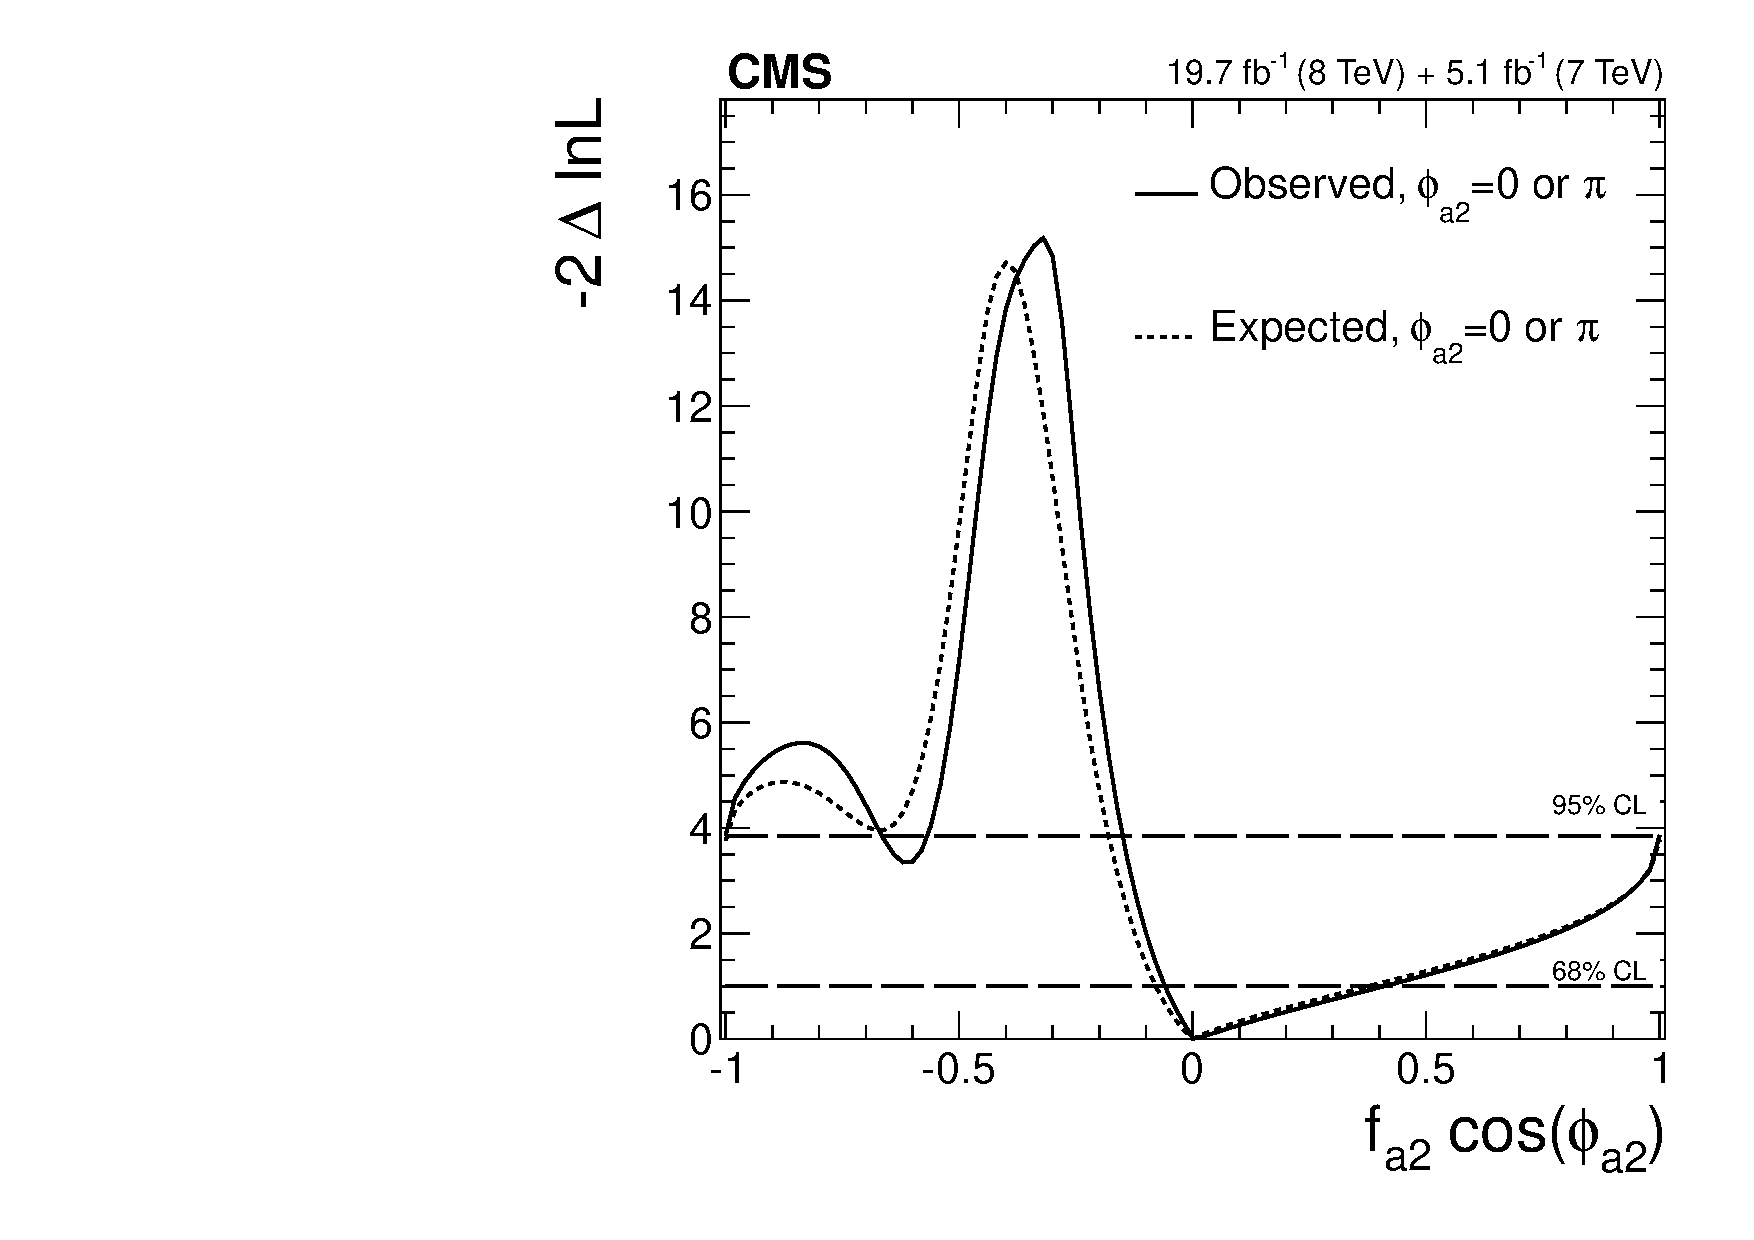
\includegraphics[width=0.31\linewidth,angle=0]{figures/fa2_Real.pdf}
%%        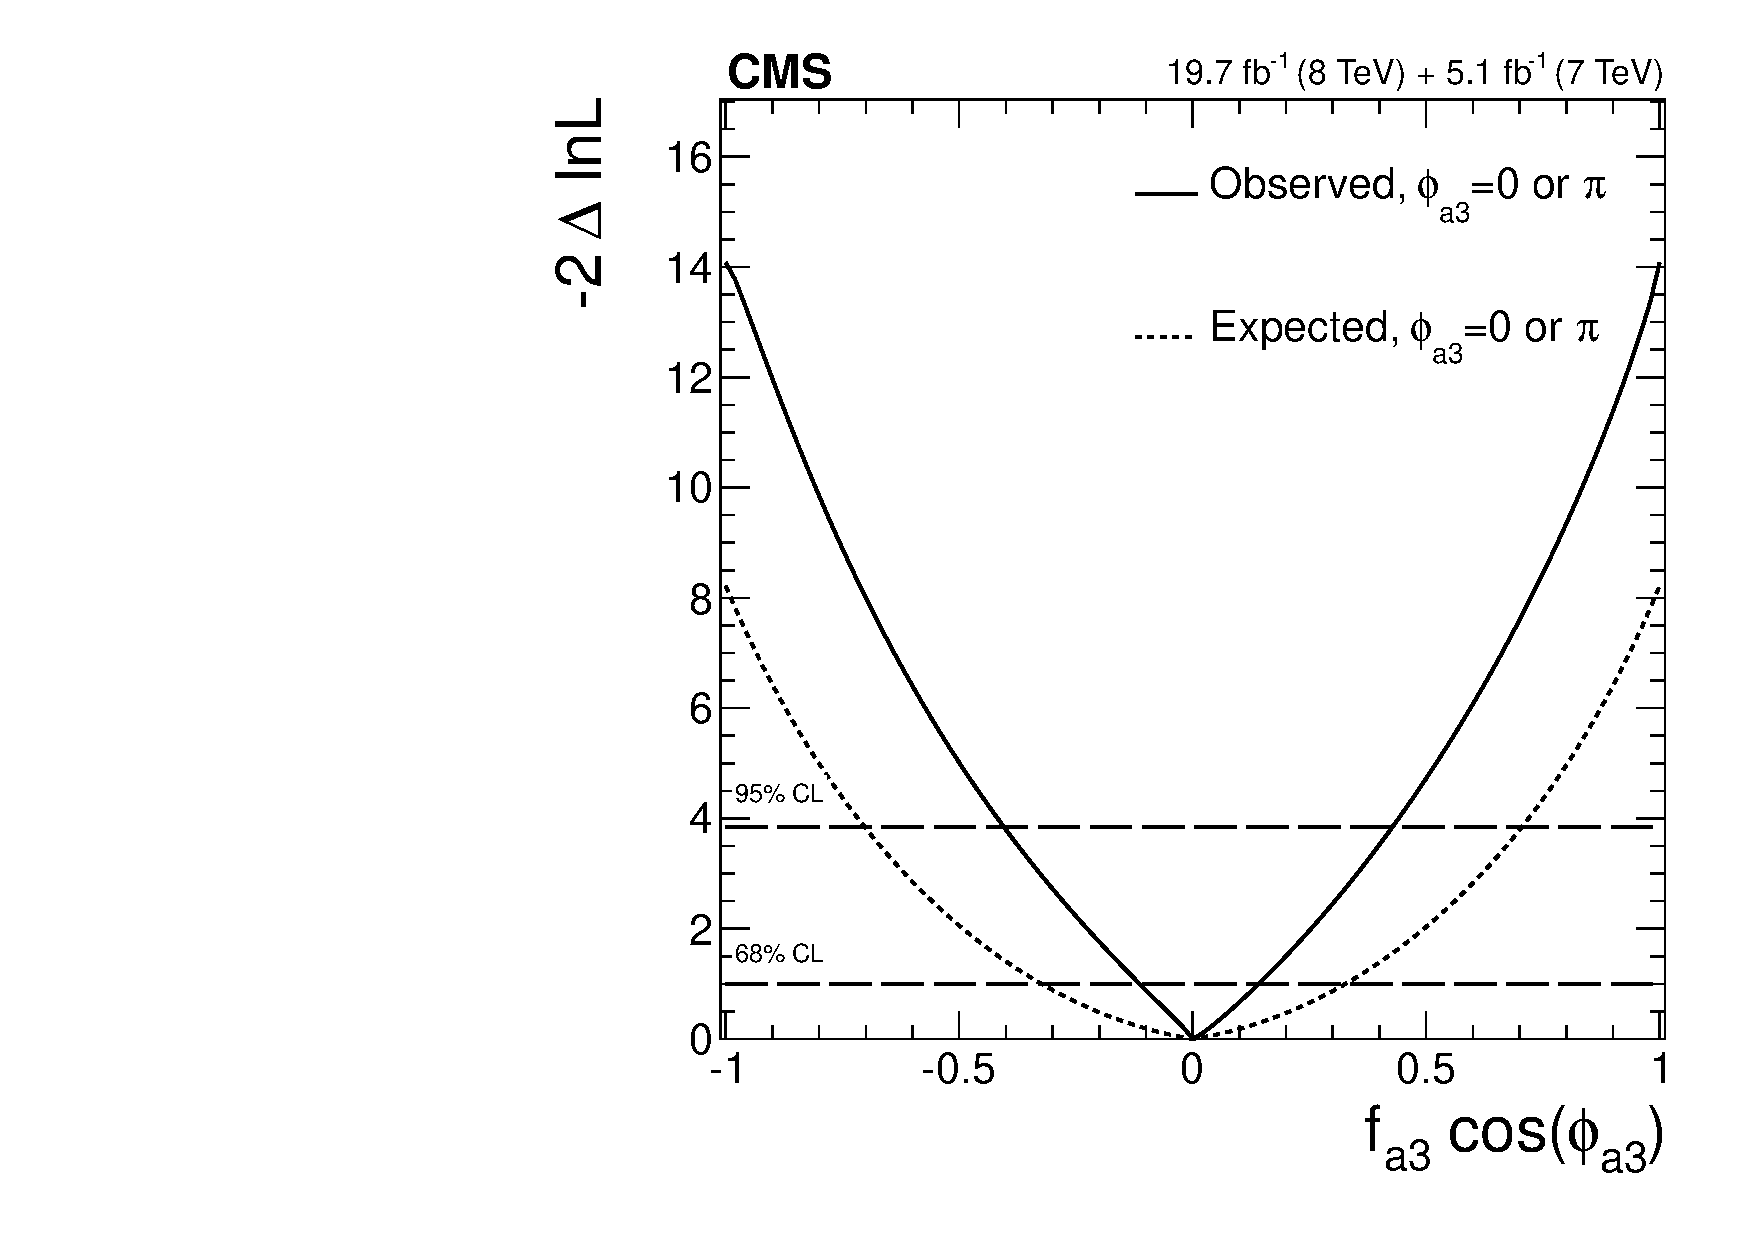
\includegraphics[width=0.31\linewidth,angle=0]{figures/fa3_Real.pdf}
%%         \caption{
%%         Expected (dashed) and observed (solid) likelihood scans using the template method for 
%%         the effective fractions $f_{\Lambda1}$, $f_{a2}$, $f_{a3}$ (from left to right) describing $\PH\PZ\PZ$ interactions. 
%%         The plots show the results when the couplings studied are constrained to be real and all other couplings are fixed to the SM predictions. 
%%         The $\cos\phi_{ai}$ term allows a signed quantity where $\cos\phi_{ai}=-1$ or $+1$.
%%         \label{fig:results_ZZ_1D}
%%         }
%% \end{center}
%% \end{figure}
%%%%%%%%%%%%%%%%%%%%%%%%%


  \item Simultaneous measurement of more than one-anomalous coupling.
    One possibility is fitting one parameter and leaving another one
    to be unconstrained, in the full allowed parameter space, with
    $0\le f_{ai}\le 1$, in the hypothesis of real couplings. This
    tests the possible simultaneous presence of more than one
    anomalous contribution to the amplitude of
    Eq.~(\ref{eq:formfact-fullampl-spin0}), without assumptions on one
    of them. Results are consistent with SM-only amplitude: the
    two-dimensional scans of the likelihood in the case of real phases
    are shown in Fig.~\ref{fig:results_ZZ_2D} (top). All other
    parameters are constrained to be the SM ones. The measurements of
    $f_{a2}$ and $f_{a3}$ are also performed with the 8-dimensional
    likelihood, yielding to a consistent result.
\item The same simultaneous measurements can be performed in the case
  of generic phases, resulting in weaker constraints, but with fewer
  assumptions. Likelihood scans for three pairs of couplings with
  generic phases are shown in Fig.~\ref{fig:results_ZZ_2D} (bottom).

%%%%%%%%%%%%%%%%%%%%%%%%%
\begin{figure}[!htbp]
\begin{center}
        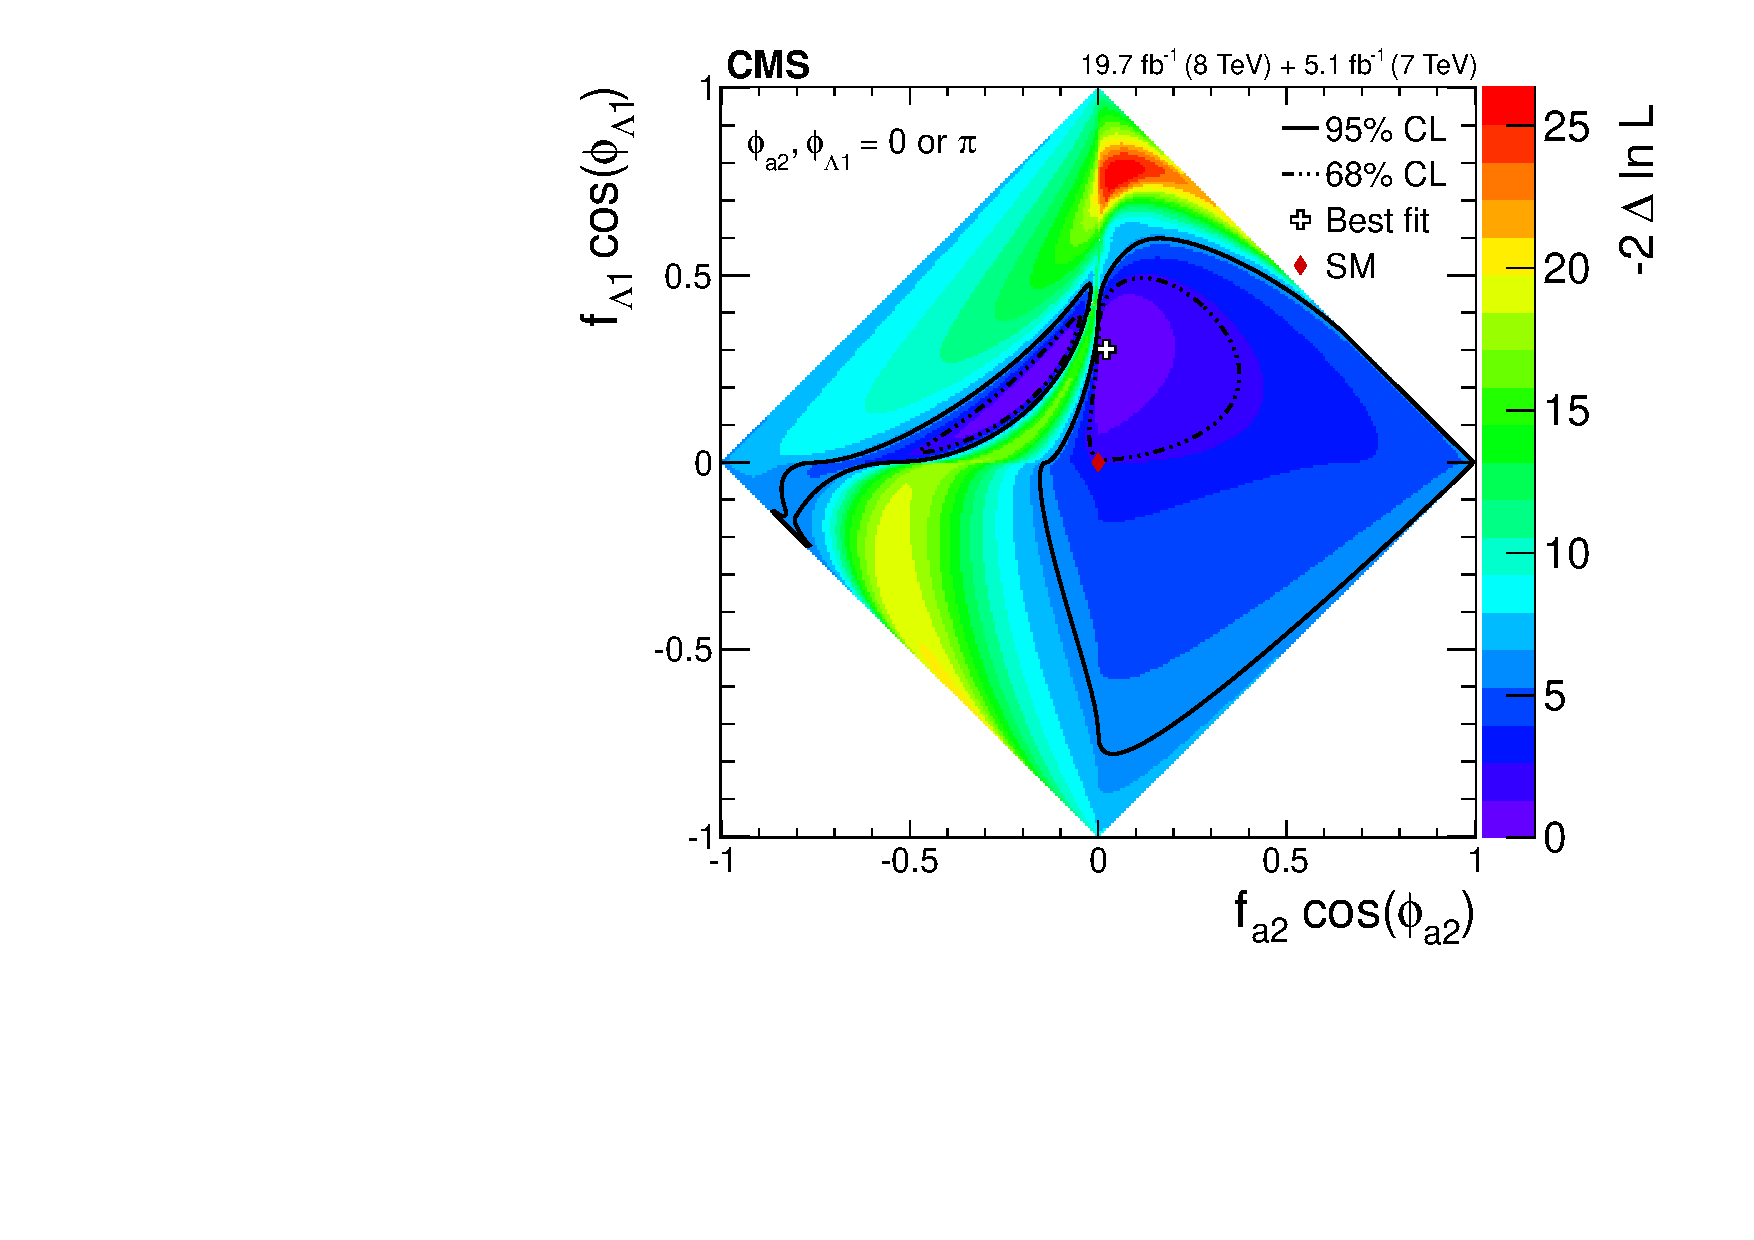
\includegraphics[width=0.31\linewidth,angle=0]{figures/fL1_vs_fa2_Real.pdf}
        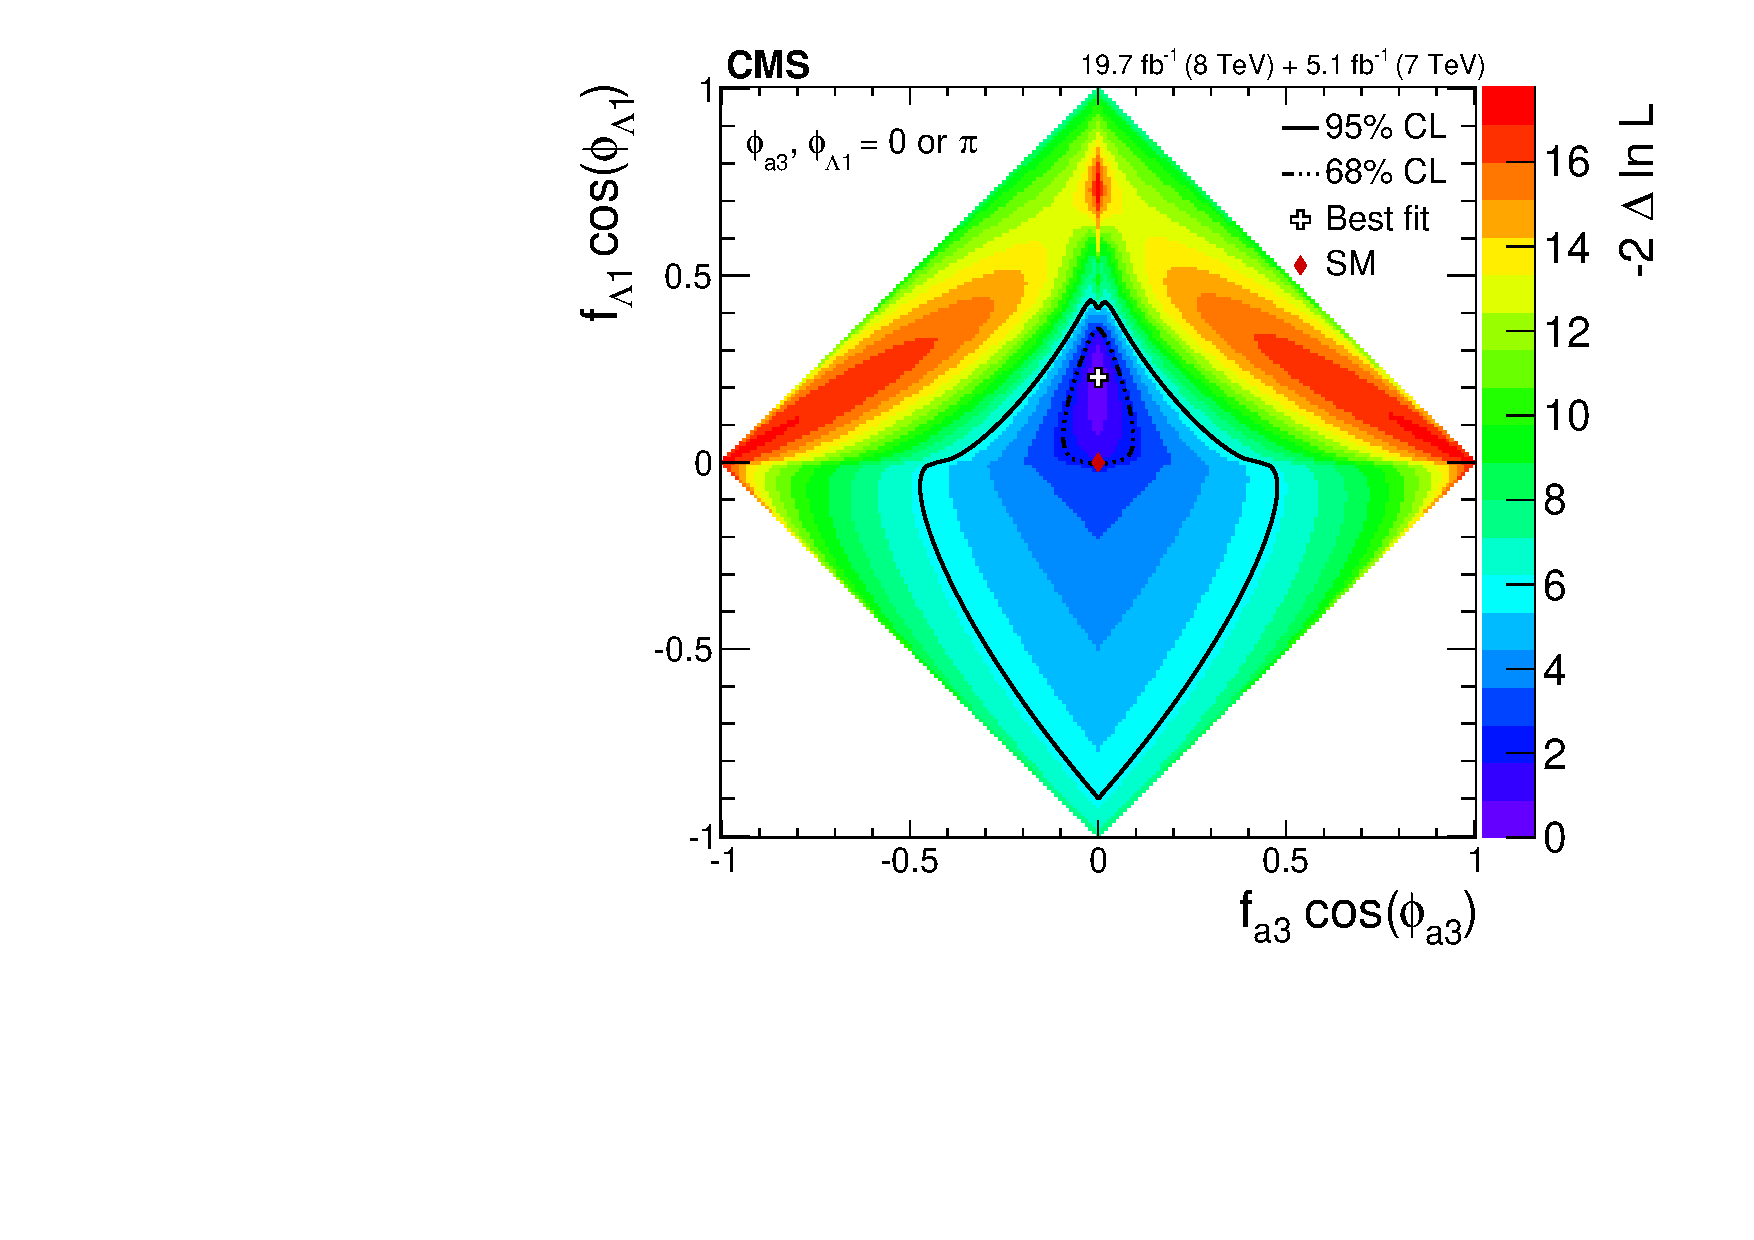
\includegraphics[width=0.31\linewidth,angle=0]{figures/fL1_vs_fa3_Real.pdf}
        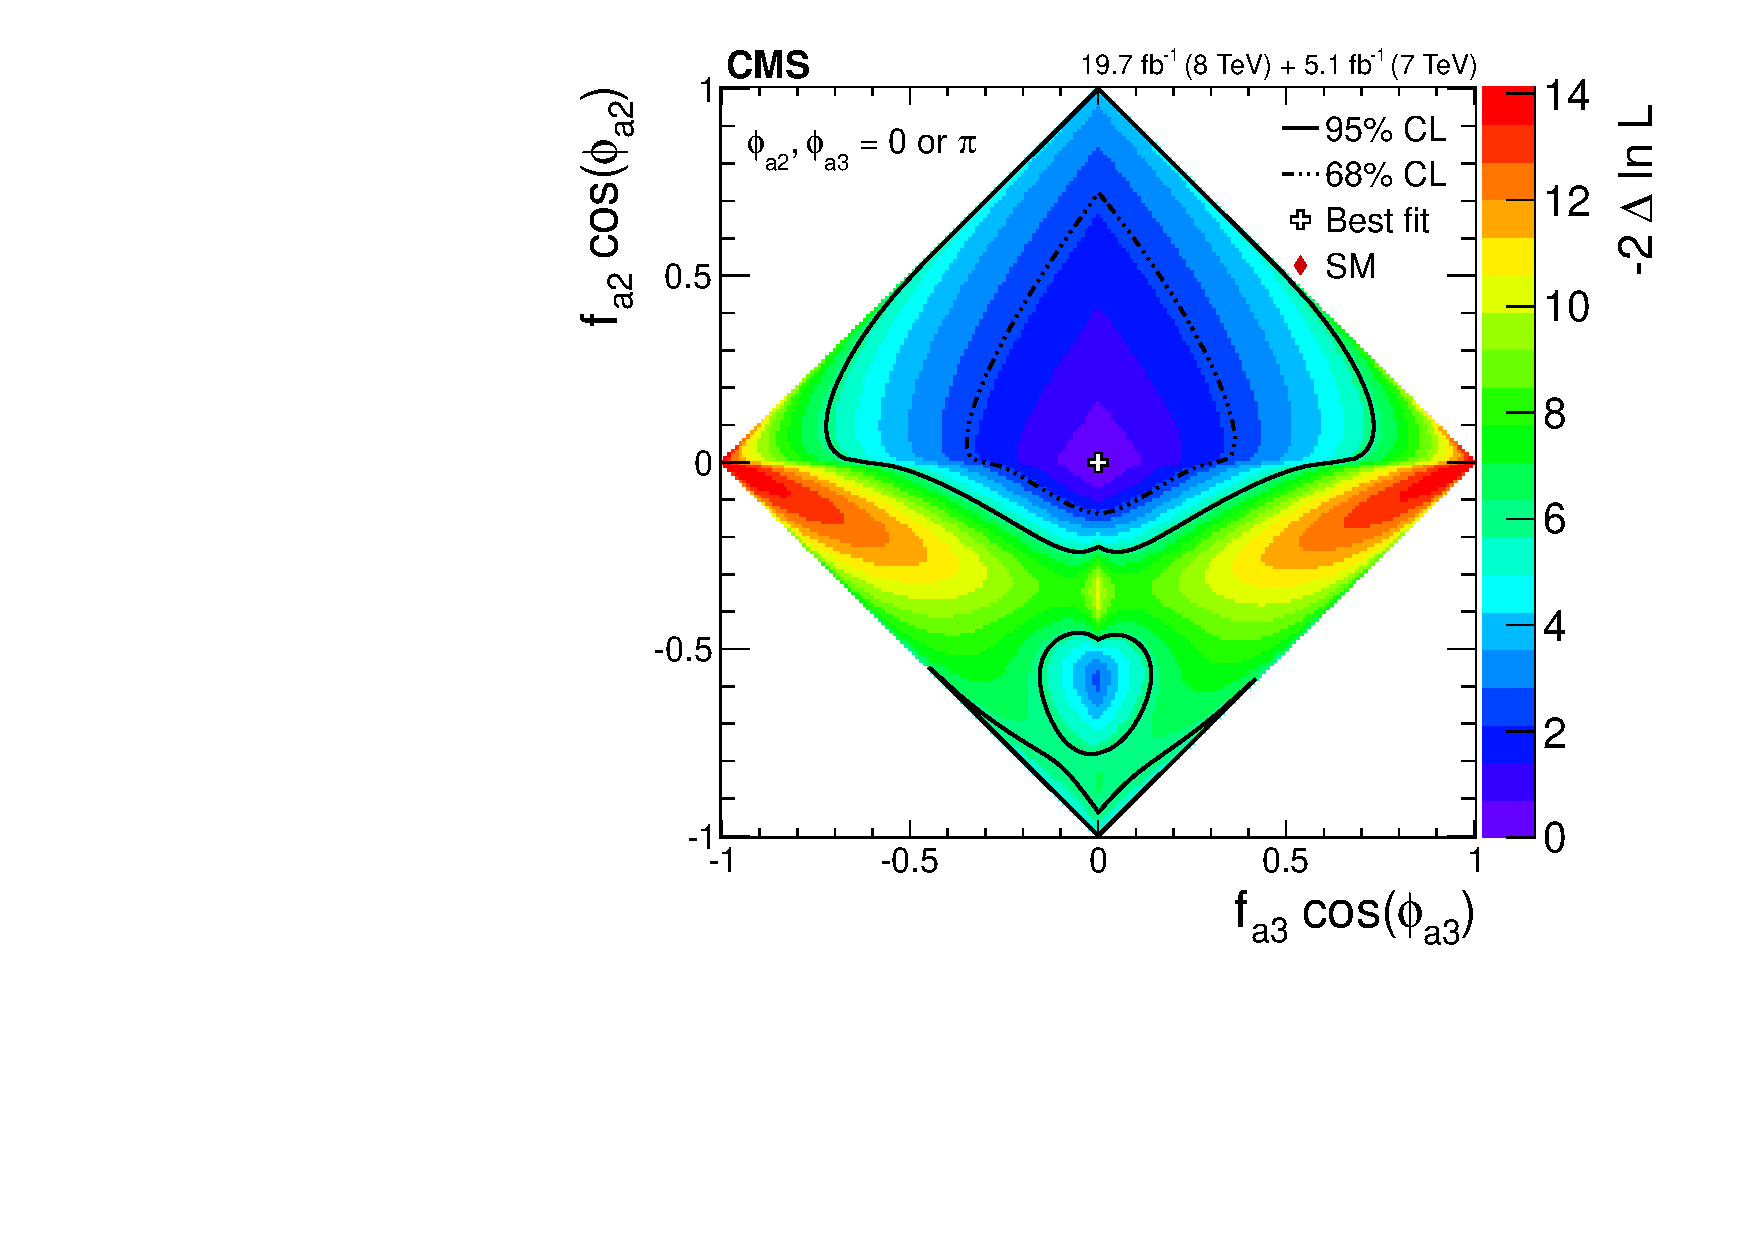
\includegraphics[width=0.31\linewidth,angle=0]{figures/fa2_vs_fa3_Real.pdf} \\
        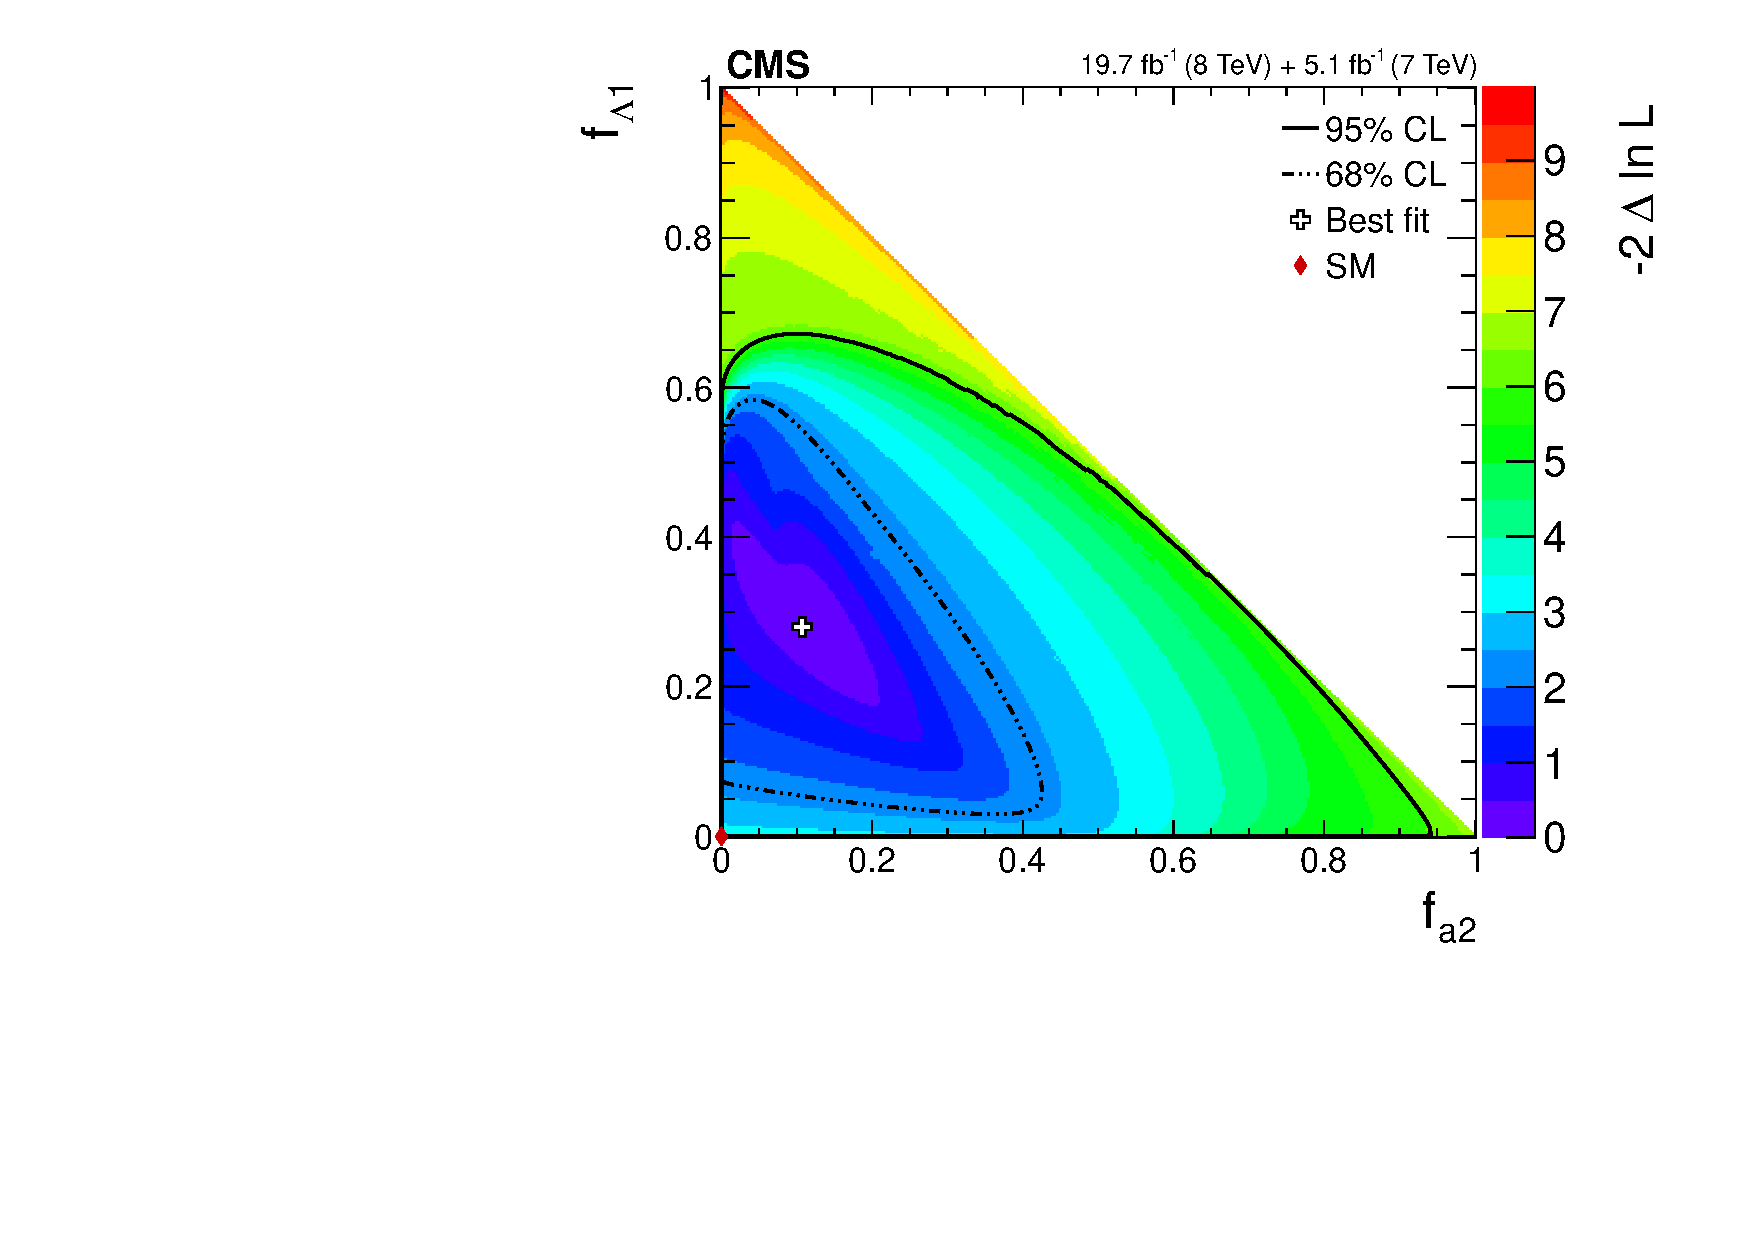
\includegraphics[width=0.31\linewidth,angle=0]{figures/fL1_vs_fa2_Profile.pdf}
        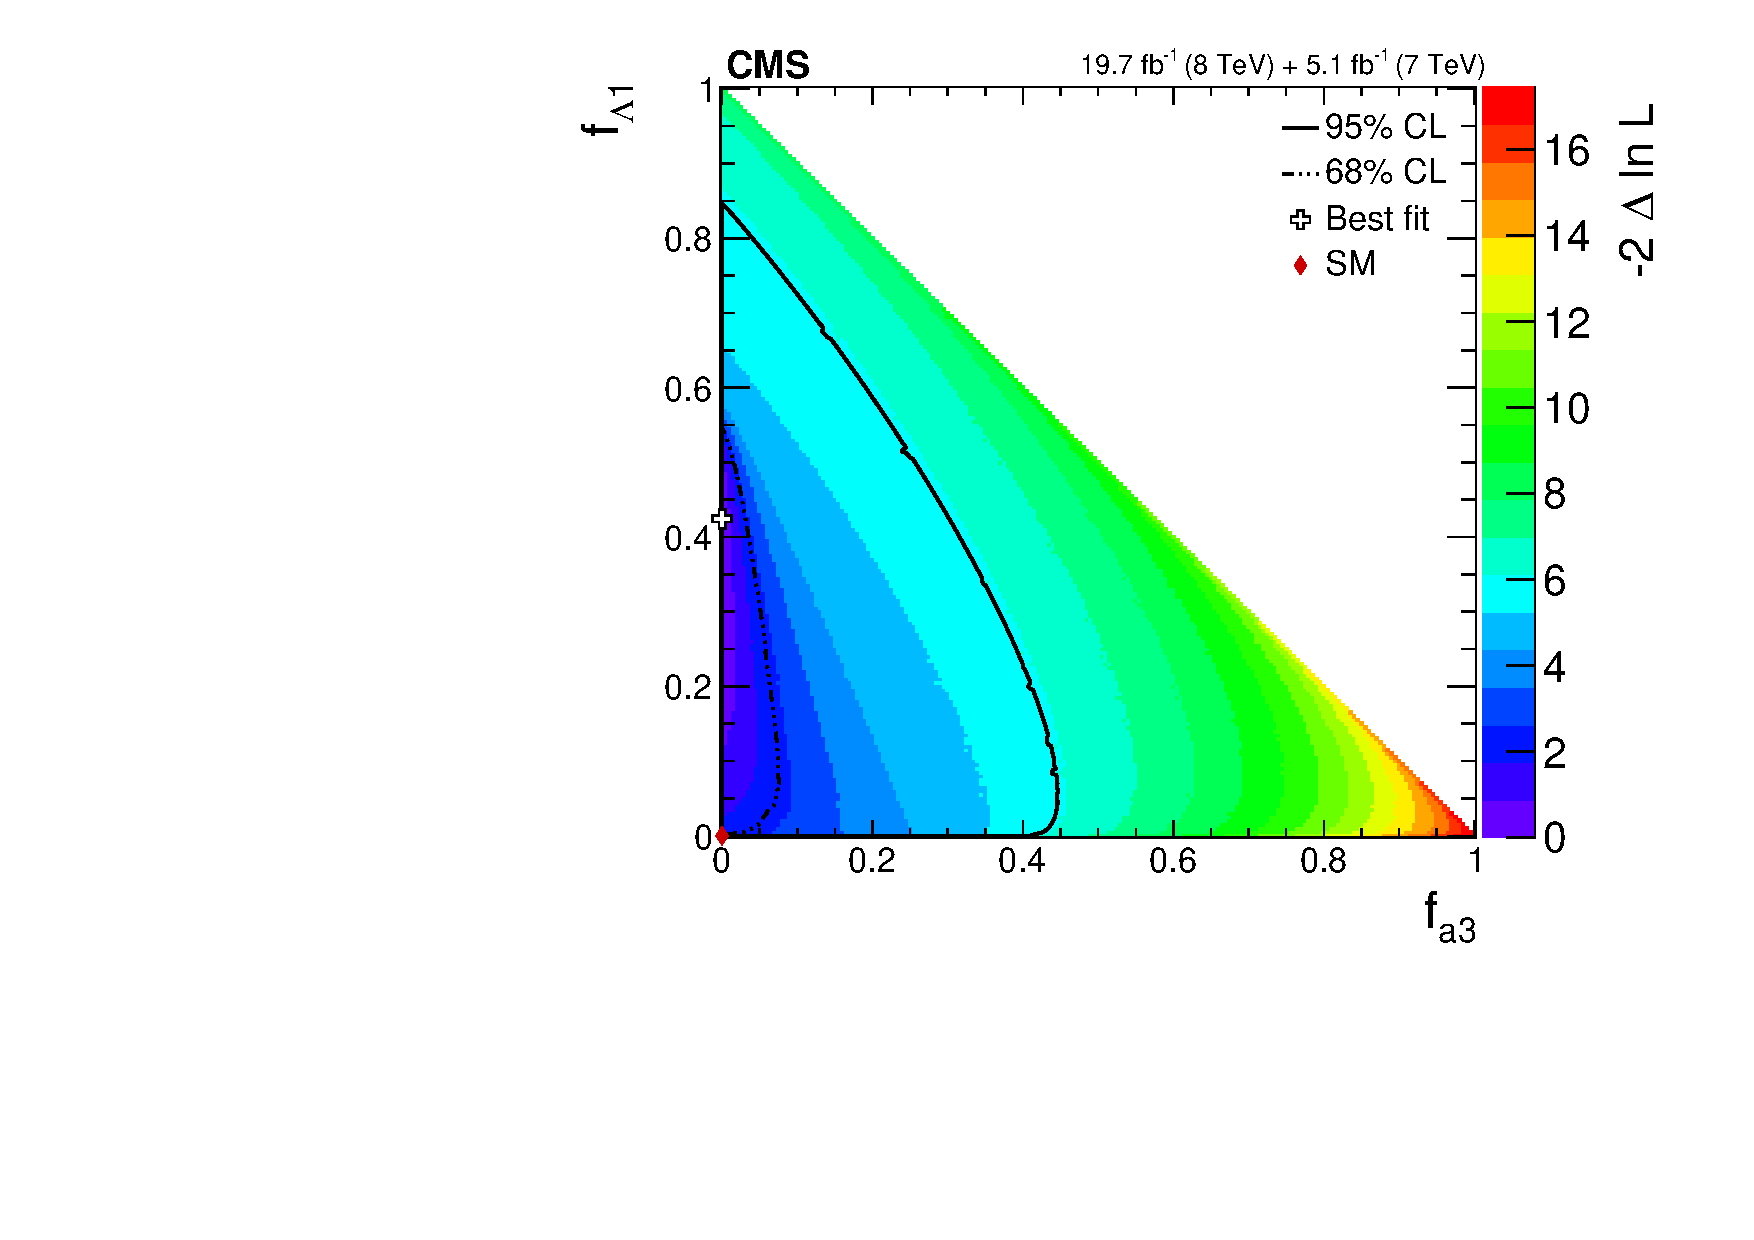
\includegraphics[width=0.31\linewidth,angle=0]{figures/fL1_vs_fa3_Profile.pdf}
        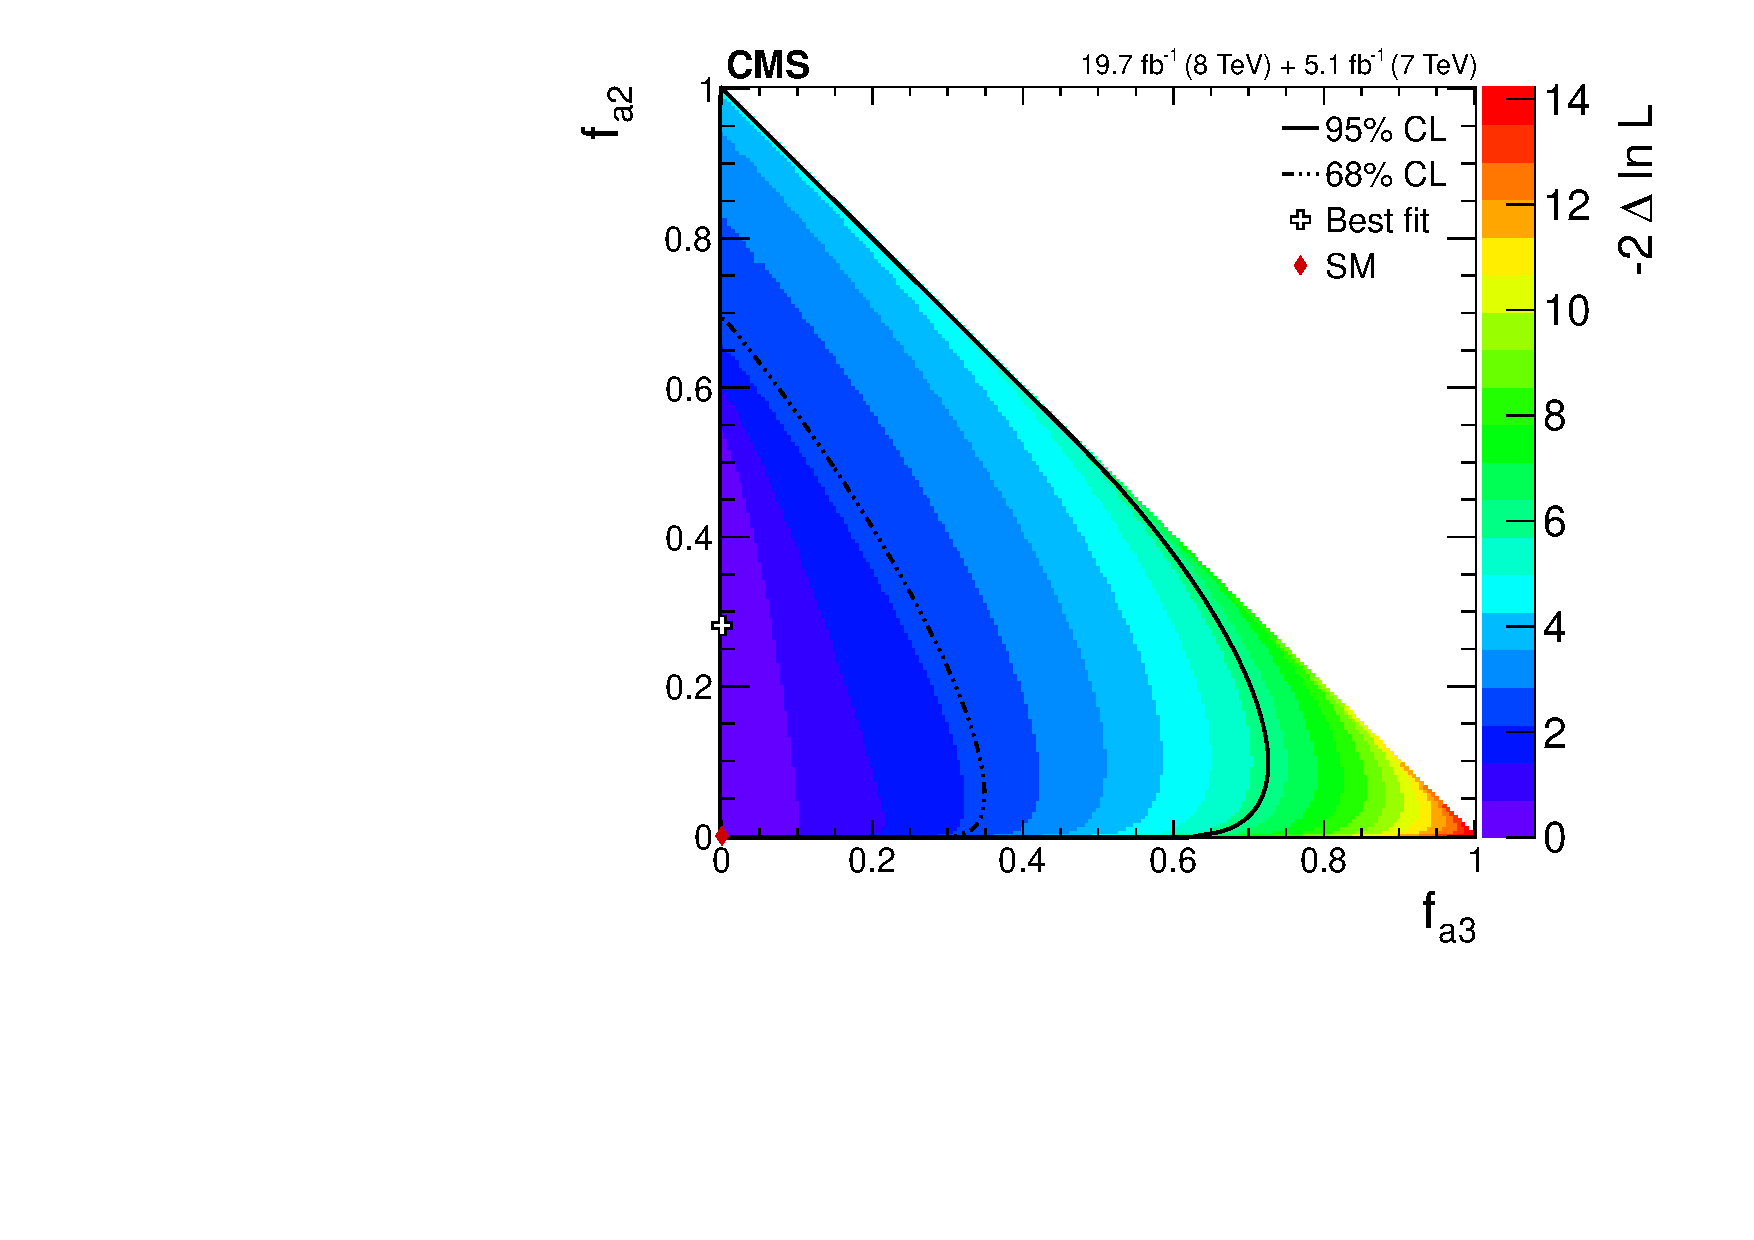
\includegraphics[width=0.31\linewidth,angle=0]{figures/fa2_vs_fa3_Profile.pdf}
        \caption{
        Observed likelihood scans using the template method for pairs of effective fractions $f_{\Lambda1}$ vs. $f_{a2}$, 
        $f_{\Lambda1}$ vs. $f_{a3}$, and $f_{a2}$ vs. $f_{a3}$ (from top to bottom) describing $\PH\PZ\PZ$ interactions. 
        The left column shows the results where the studied couplings are constrained to be real
        and all other couplings are fixed to the SM predictions.
        The right column shows the results when the phases of the anomalous couplings are left unconstrained. 
        \label{fig:results_ZZ_2D}
        }
\end{center}
\end{figure}
%%%%%%%%%%%%%%%%%%%%%%%%%

\end{enumerate}

The same set of measurements, presented for the $\chanHZZ$, can be
performed in the $\chanHWW$, though with reduced sensitivity, due to
the fewer kinematic observables available, and finally combined
together. For the latter, only real couplings, $\phi_{ai}^{\PW\PW}=0$
or $\pi$, are considered. The combination can be performed in two
scenarios, assuming custodial symmetry ($a_1^{WW} = a_1$), or not
assuming any ratio between the two scenarios. In the first case, the
relationships between the yield of $\chanHZZ$ and $\chanHWW$ yields to
a stronger constraint ont the anomalous couplings.
The likelihood scan for a particular value of $R_{ai}=0.5$ $(r_{ai} = 1)$
is shown in Fig.~\ref{fig:hwwscans}, where the stronger constraint from 
the yield relationship between the two channels is visible. When the custodial
symmetry is assumed, an even stronger constraint arise, strongly disfavouring 
the hypothesis of $f_{a2}=\pm1$.
%

%%%%%%%%%%%%%%%%%%%%%%%
\begin{figure}[!htbp]
  \begin{center} 
    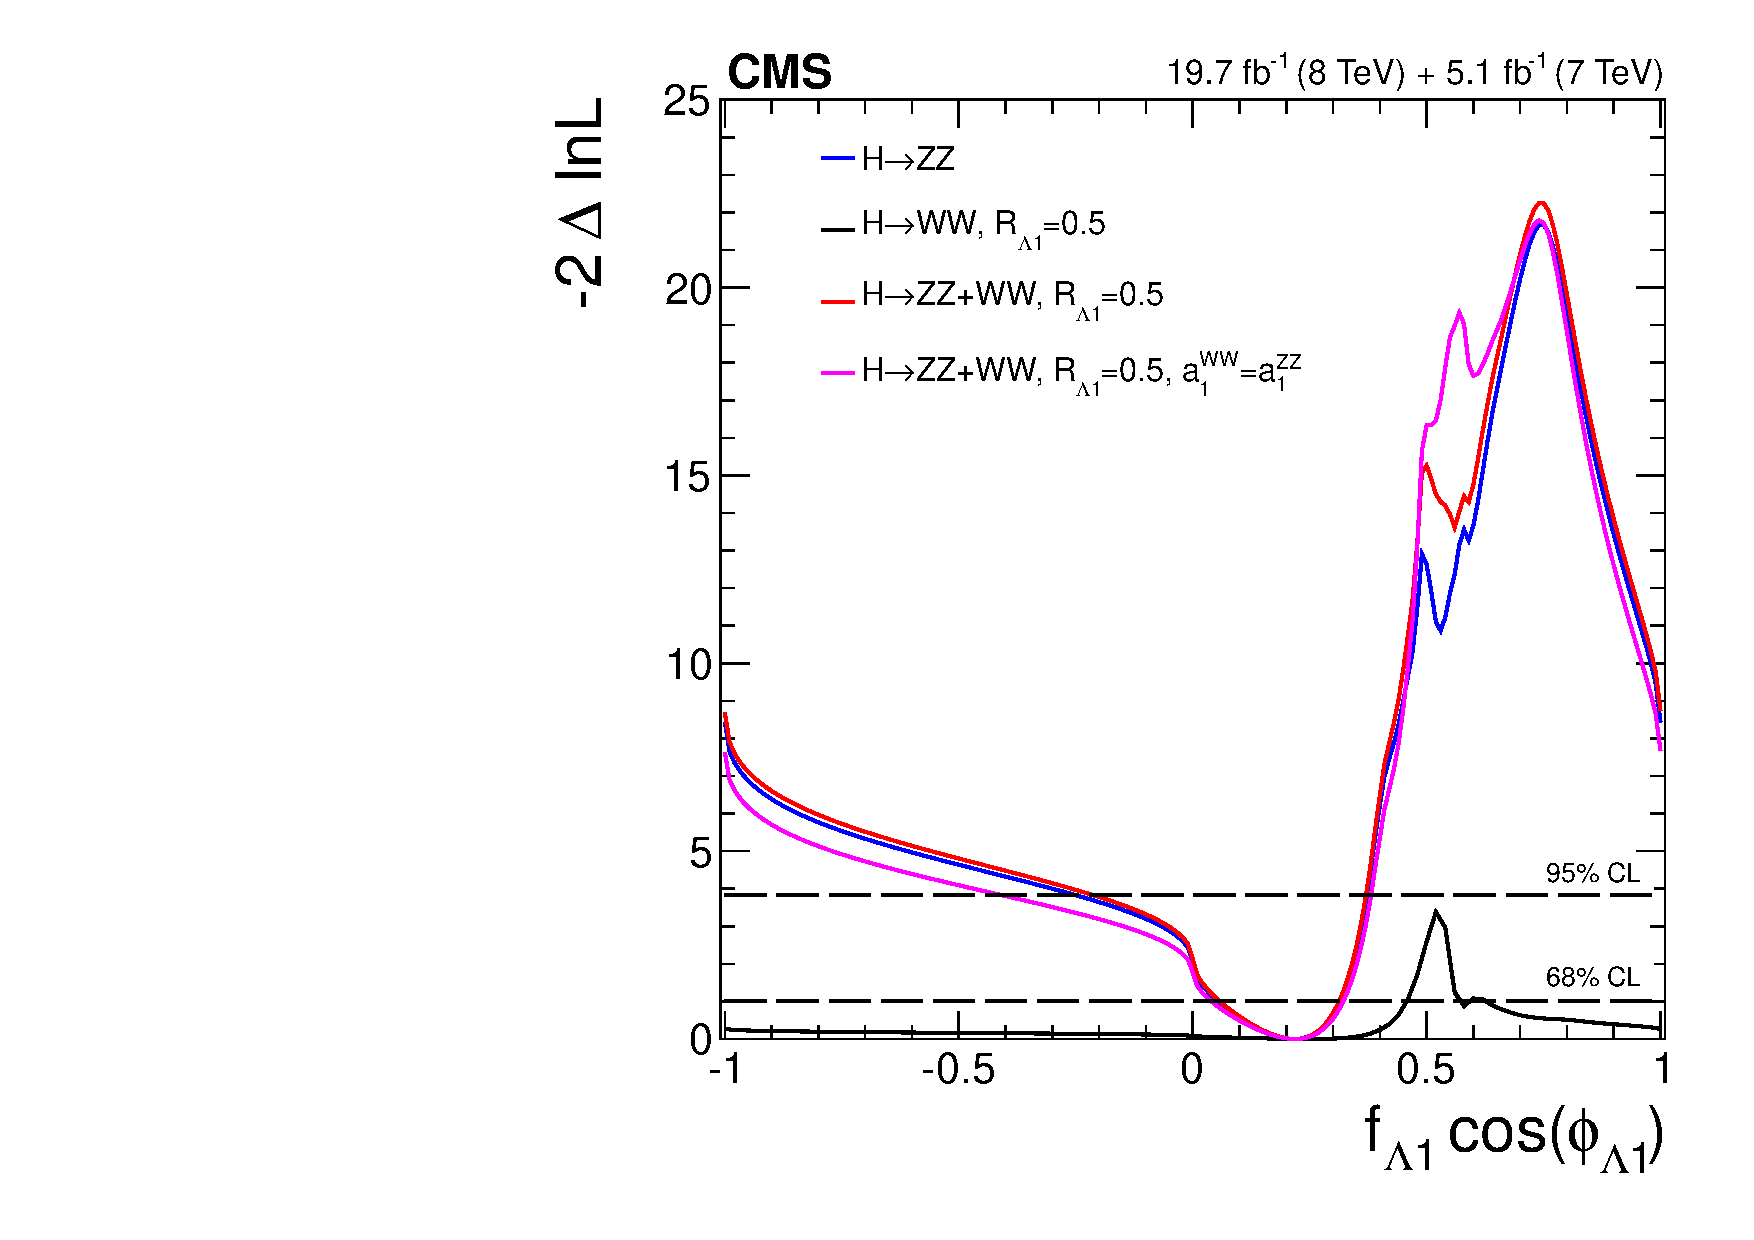
\includegraphics[width=0.31\linewidth]{figures/flambda1_combine_ww.pdf}
    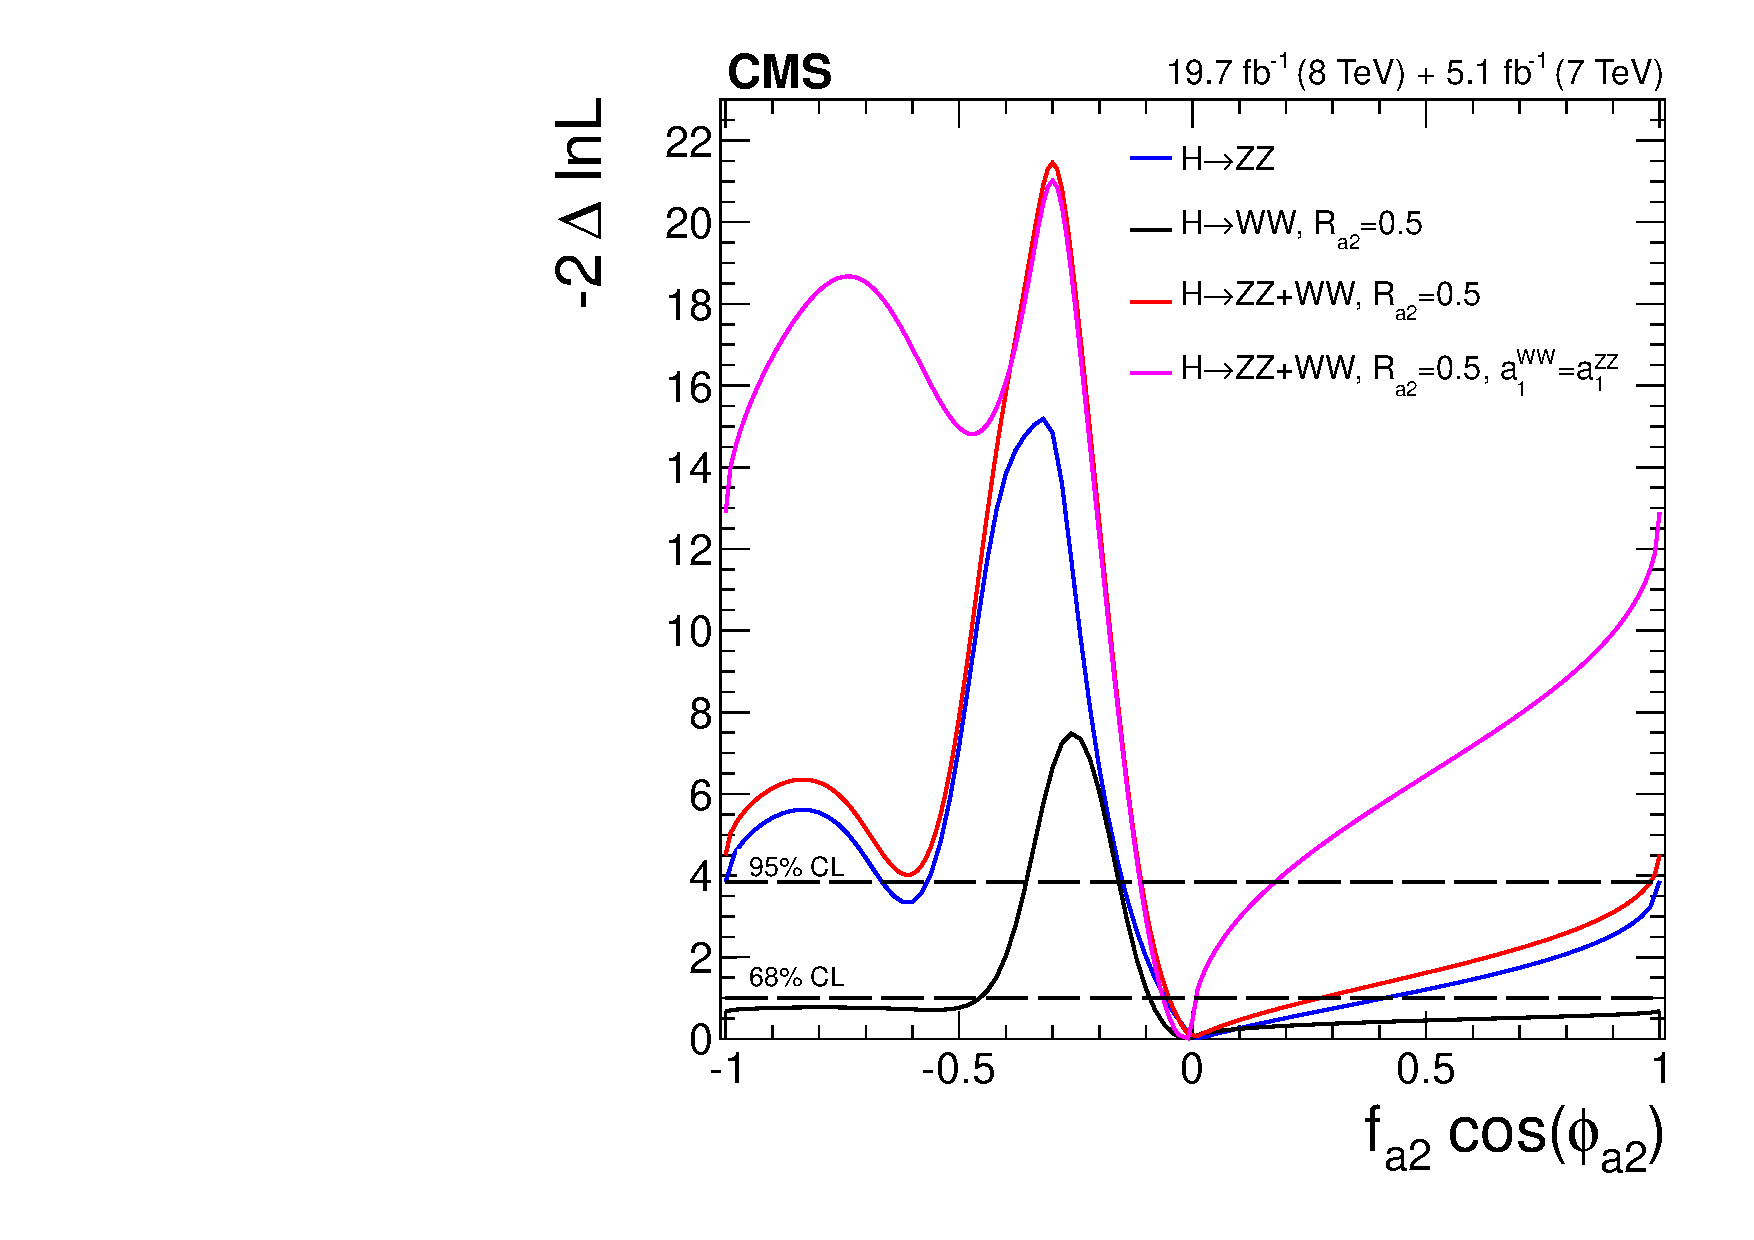
\includegraphics[width=0.31\linewidth]{figures/fa2_combine_ww.pdf}
    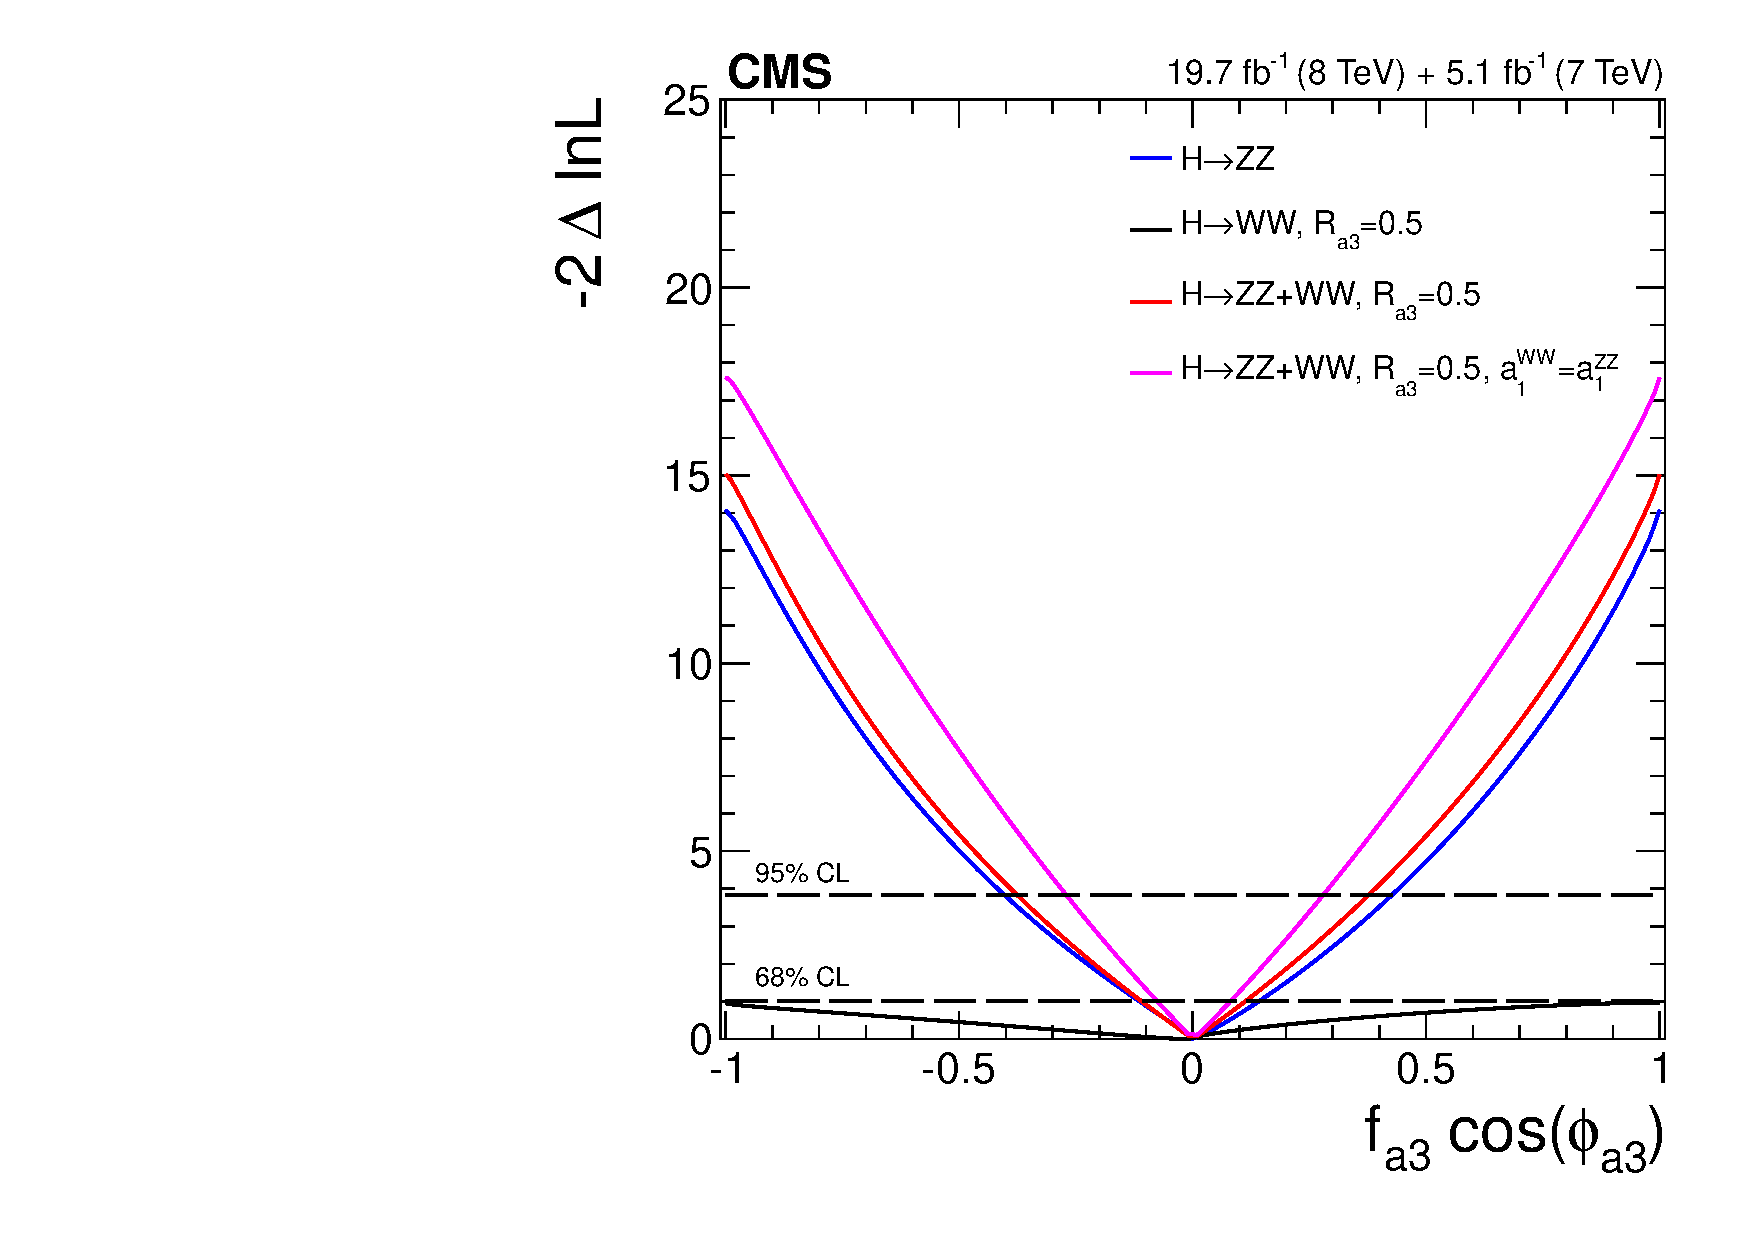
\includegraphics[width=0.31\linewidth]{figures/fa3_combine_ww.pdf}
    \caption{
      Expected and observed likelihood scans for effective fractions 
      $f_{\Lambda1}$ (left), $f_{a2}$ (middle), $f_{a3}$ (right). 
      The couplings studied are constrained to be real and all other anomalous couplings are fixed to the SM predictions. 
      The $\cos\phi_{ai}$ term allows a signed quantity where $\cos\phi_{ai}=-1$ or $+1$.
      The plots show the combined  $\PH\to\PW\PW$ and $\PH\to\PZ\PZ$ result in terms of the $\PH\PZ\PZ$ couplings for $R_{ai} = 0.5$. 
      Measurements are shown for each channel separately and two types of combination are present:
      using $a_1^{\PW\PW} = a_1$ (red) and without such a constraint (magenta).
    \label{fig:hwwscans}
    }
  \end{center}
\end{figure}
%%%%%%%%%%%%%%%%%%%%%%%

%
Overall, all anomalous $\PH\V\V$ couplings are found to be consistent
with zero, which is also consistent with the expectation from the SM
where these couplings are expected to be very small, well below the
current sensitivity.


\section{Conclusions}
\label{sec:conclusions}
In this conference the study of a the Higgs boson spin-parity
properties have been presented, through its decays into two
electroweak gauge bosons: $\PH\to\PZ\PZ$, $\PZ \Pgs$,
$\Pgs\Pgs\to4\ell$, $\PH\to\PW\PW\to\ell\nu\ell\nu$ and
$\PH\to\Pgg\Pgg$ decay modes.

For the decays into two massive gauge bosons, $\PZ$ or $\PW$, the
tensor structure of its interactions is studied, for the presence of
anomalous couplings with $\PZ\PZ$ and $\PW\PW$ bosons under spin-zero,
-one, and -two hypotheses. The combination of the results in the two
decay channels leads to a strong constraint on the anomalous
$\PH\to\V\V$ interactions. The $\chanHgg$ allows to put further
constraints on the spin-two hypothesis.

The exotic-spin boson is tested for mixed-parity spin-one states and
ten spin-two hypotheses The spin-one hypotheses are excluded at
greater than 99.99\% CL, the spin-two boson with gravity-like minimal
couplings is excluded at 99.9\% CL, and the other spin-two hypotheses
tested are excluded at 99\% CL or higher, both with production
dependent and independent analyses. 
%
For this reason, the study concentrates on the measurement of eleven
anomalous couplings to the $\PH\PZ\PZ$, $\PH\PZ\Pgg$,
$\PH\Pgg\Pgg$, and $\PH\PW\PW$ interactions under the assumption of
a spin-zero Higgs boson. All observations are consistent with the
expectations for a scalar SM-like Higgs boson.



%% The Appendices part is started with the command \appendix;
%% appendix sections are then done as normal sections
%% \appendix

%% \section{}
%% \label{}

%% References
%%
%% Following citation commands can be used in the body text:
%% Usage of \cite is as follows:
%%   \cite{key}         ==>>  [#]
%%   \cite[chap. 2]{key} ==>> [#, chap. 2]
%%

%% References with BibTeX database:
%\nocite{*}
\bibliographystyle{elsarticle-num}
\bibliography{emanueledimarco}


%% Authors are advised to use a BibTeX database file for their reference list.
%% The provided style file elsarticle-num.bst formats references in the required Procedia style

%% For references without a BibTeX database:

% \begin{thebibliography}{00}

%% \bibitem must have the following form:
%%   \bibitem{key}...
%%

% \bibitem{}

% \end{thebibliography}

\end{document}

%%
%% End of file `nuphbp-template.tex'. 
